%% This is an example first chapter.  You should put chapter/appendix that you
%% write into a separate file, and add a line \include{yourfilename} to
%% main.tex, where `yourfilename.tex' is the name of the chapter/appendix file.
%% You can process specific files by typing their names in at the 
%% \files=
%% prompt when you run the file main.tex through LaTeX.

\chapter{Integrating archival tag data and a high-resolution oceanographic model to estimate basking shark (\textit{Cetorhinus maximus}) movements in the western Atlantic}
\label{chap:3}
\raggedbottom
%\begin{singlespace}
%Camrin D. Braun1,2*, Gregory B. Skomal3, Simon R. Thorrold2
	%Massachusetts Institute of Technology-Woods Hole Oceanographic Institution Joint Program in %Oceanography/Applied Ocean Science and Engineering, Cambridge, MA 02139
	%Biology Department, Woods Hole Oceanographic Institution, Woods Hole, MA 02540
	%Massachusetts Division of Marine Fisheries, New Bedford, MA 02744, USA

%*corresponding author: cbraun@whoi.edu; +1 5082893961
%Keywords: movement ecology; satellite archival telemetry; migration; mesopelagic; oceanographic modeling; %site fidelity


%\\
{\let\thefootnote\relax\footnotetext{This chapter was originally published as Braun, C.D., Skomal, G.B., and Thorrold S.R. (2018). \href{https://www.frontiersin.org/articles/10.3389/fmars.2018.00025/full}{Integrating archival tag data and a high-resolution oceanographic model to estimate basking shark (\textit{Cetorhinus maximus}) movements in the western Atlantic.} \emph{Frontiers in Marine Science} 5: 25. }}
%\end{singlespace}
{\let\thefootnote\relax\footnotetext{G.B.S. and S.R.T. designed the study and conducted the tagging; C.D.B. performed the analysis and wrote the paper. G.B.S. and S.R.T. contributed to the writing of the paper.}}
%{\let\thefootnote\relax\footnotetext{The supplemental figures, tables, and data sheets for this chapter can be found in \cref{sec:app3}.}}

\clearpage

\section{Abstract}

Basking shark (\textit{Cetorhinus maximus}) populations are considered "vulnerable" globally and "endangered" in the northeast Atlantic by the International Union for the Conservation of Nature. Much of our knowledge of this species comes from surface observations in coastal waters, yet recent evidence suggests the majority of their lives may be spent in the deep ocean. Depth preferences of basking sharks have significantly limited movement studies that used pop-up satellite archival transmitting (PSAT) tags as conventional light-based geolocation is impossible for tagged animals that spend significant time below the photic zone. We tagged 57 basking sharks with PSAT tags in the NW Atlantic from 2004-2011. Many individuals spent several months at meso- and bathy-pelagic depths where accurate light-level geolocation was impossible during fall, winter and spring. We applied a newly-developed geolocation approach for the PSAT data by comparing three-dimensional depth-temperature profile data recorded by the tags to modeled in-situ oceanographic data from the high-resolution HYbrid Coordinate Ocean Model (HYCOM). Observation-based likelihoods were leveraged within a state-space hidden Markov model (HMM). The combined tracks revealed that basking sharks moved from waters around Cape Cod, MA to as far as the SE coast of Brazil (20$^{\circ}$S), a total distance of over 17,000 km. Moreover, 59\% of tagged individuals with sufficient deployment durations (> 250 days) demonstrated seasonal fidelity to Cape Cod and the Gulf of Maine, with one individual returning to within 60 km of its tagging location one year later. Tagged sharks spent most of their time at epipelagic depths during summer months around Cape Cod and in the Gulf of Maine. During winter months, sharks spent extended periods at depths of at least 600 m while moving south to the Sargasso Sea, the Caribbean Sea, or the western tropical Atlantic. Our work demonstrates the utility of applying advances in oceanographic modeling to understanding habitat use of highly migratory, often meso- and bathy-pelagic, ocean megafauna. The large-scale movement patterns of tagged sharks highlight the need for international cooperation when designing and implementing conservation strategies to ensure that the species recovers from the historical effects of over-fishing throughout the North Atlantic Ocean.

\section{Introduction}
The basking shark, \textit{Cetorhinus maximus} (Gunnerus 1765), is the second largest fish species, attaining weights of up to 4 tonnes and lengths up to 12 m \citep{Sims2008}. It is known to inhabit boreal to tropical \citep{Skomal2009} waters circumglobally and is most often observed on continental shelves \citep{Sims2006}. Despite its size and widespread distribution, major gaps in our understanding of basking shark ecology remain. Population size and structure are currently unresolved and information about fisheries interactions is limited \citep{Sims2008}. Although there is evidence to suggest population recovery in some areas following exploitation \citep{Witt2012}, the lack of information about key life history traits, population size, movements, and habitat use is problematic as global anthropogenic pressures on elasmobranchs continue to rise \citep{Dulvy2008, Ferretti2010}.

Basking sharks exhibit life history characteristics that make them particularly vulnerable to exploitation, including low fecundity, slow growth and maturity, and long gestation times \citep{Compagno1984, Sims2008}. There is, therefore, concern over the status of basking shark populations worldwide, and the species is listed on Appendix II of the Convention on the International Trade in Endangered Species (CITES) and Appendices I and II of the Convention for the Conservation of Migratory Species of Wild Animals (CMS). It is also considered "vulnerable" globally and "endangered" in the northeast Atlantic by the International Union for the Conservation of Nature (IUCN).

Historically, information on the ecology of large pelagic animals has been limited to scarce observations that are limited geographically \citep{Templeman1963, SquireJr1990, Francis2002}. Almost all of our knowledge of basking shark ecology, for instance, comes from surface observations in coastal waters \citep{Sims2006, Sims2008}.  Yet recent evidence from electronic archival tags suggests that perhaps the majority of their lives are spent offshore at depths below the euphotic zone \citep{Skomal2009}. Indeed, the rapid development of electronic tag technologies has provided a powerful means of gaining detailed information about the behavior of marine species \citep{Block2011}. PSAT tags have been particularly helpful in ocean environments as data are relayed back to the researcher via satellite upon tag release from the individual \citep[\emph{e.g.}][]{Block2011}. These tags have provided a wealth of information on sharks \citep{Werry2014, Berumen2014}, rays \citep{Braun2014, Thorrold2014a}, and large teleost fishes \citep{Braun2015a} by eliminating the need to physically recover the tag at the end of the deployment. 

While electronic tags have revolutionized the study of movement ecology in the ocean, a significant hurdle remains when attempting to track marine fishes compared with terrestrial counterparts.  Tags using Argos or Global Positioning System (GPS) locations require the tag antenna to break the water surface long enough for communication with satellites to be established (Argos) or a snapshot of the satellite constellation to be received (GPS). Researchers, have, therefore, relied mostly on PSAT tags that use light-level geolocation in which a threshold algorithm is used to detect solar altitude above the horizon from which estimates of longitude (local noon) and latitude (sunrise/sunset) can be estimated \citep{Hill2001}. While sea surface temperature (SST) and bathymetry can improve these estimates \citep{Galuardi2010, Lam2010}, light-based geolocation requires occupation of the photic zone to record adequate light data for geolocation, and even estimates with quality light data can be error prone \citep{Braun2015}.  However a number of marine species rarely, if ever, experience enough downwelling light or spend adequate time at the surface to determine their position with PSAT tags \citep{Aarestrup2009, Skomal2009, Peklova2012}. Animals that spend significant time at depths below the photic zone have, therefore, proved extremely difficult to track in ocean ecosystems \citep[\emph{e.g.}][]{Skomal2009, Dewar2011}. 

The use of PSAT tags to track basking shark movements has proved particularly difficult in the northwestern Atlantic as basking sharks spend months at a time below the euphotic zone where light-based geolocation is impossible \citep{Skomal2009}.  We have recently developed a new geolocation approach that combines all the physical data collected from archival tags, including light levels and depth-temperature profiles, in a likelihood framework to more accurately track the movements of tagged fishes in the ocean \citep{Braun2018a}. Our method uses a purely diffusive animal movement model (\emph{e.g.} Brownian motion) with behavior state switching (migratory or resident states based on a priori movement speeds) coupled with observations of the environment (\emph{e.g.} in situ or modeled oceanography) to estimate the posterior distribution of the state (\emph{e.g.} animal position and behavior) in a hidden Markov model (HMM) framework. Depth-temperature profiles provide diagnostic oceanographic signatures that, along with other data sources like light, SST, and maximum depth, may be leveraged to help constrain position \citep{Aarestrup2009, Skomal2009}.

Satellite tags have been deployed on basking sharks in the Atlantic since the pioneering work of \cite{Priede1984}. Yet, basking shark movements and ecology remain poorly understood. Here, we present the results of an intensive tagging effort that deployed 57 PSAT tags on adult basking sharks during summer months in waters adjacent to Cape Cod, Massachusetts. Profiles recorded by the tags were integrated with high-resolution oceanographic model outputs and in situ climatological data to construct likelihoods and improve geolocation estimates for basking sharks. The data provide a rare assessment of the large-scale movements and migratory behavior of the ocean's second largest fish.  The information is, in turn, a prerequisite for any attempts to estimate abundance and population structure of basking sharks in the Atlantic Ocean.

\section{Methods}
\subsection{Study area and tagging}
We opportunistically deployed a variety of PSAT tags on basking sharks near Cape Cod, Massachusetts (USA) in the Northwest Atlantic (NWA) between 2004 and 2011 (\cref{tab:c3t1}). Total length of each individual was estimated relative to the tagging vessel and, where possible, the pelvic region was visually inspected to determine sex. Tags were applied by a professional harpoon fisherman into the dorsal musculature near the base of the first dorsal fin \citep{Chaprales1998}. This research was performed in accordance with the Woods Hole Oceanographic Institution's Animal Care and Use Committee (IACUC) protocol \#16518.

\subsection{Tag types}
Three types of PSAT tags were deployed on basking sharks (\cref{tab:c3t1}). These tags (Models Mk10-PAT, Mk10-AF, miniPAT; Wildlife Computers, Inc., WA, USA) logged depth, temperature, and light level data every 10 seconds (Mk10-AF) or 15 seconds (Mk10-PAT, miniPAT) to onboard memory. All tags recorded light data for geolocation purposes, and the Mk10-AF tag housed a Fastloc GPS receiver for acquiring high-resolution location information. Software in the tags summarized the high-resolution archived data into depth-temperature profiles at 8 depths (between minimum and maximum depth occupied for the summary period) for a 6, 12, or 24-hour period depending on tag programming. These data were compiled into a single daily summary profile for data analysis. Tags also transmitted a summary of an individual's time of occupation within designated depth or temperature bins at 6, 12, or 24-hour resolution that was also compiled into daily summaries. Depth and temperature bin number, resolution, and extent differed slightly among tag type and year of tag deployment, but all were compiled to encompass the same depth (< 10, 10-25, 25-50, 50-200, 200-400, 400-1000, > 1000 m) and temperature bins (< 7, 7-9, 9-11, 11-13, 13-15, 15-17, 17-19, 19-21, 21-23, 23-25, > 25$^{\circ}$C) for subsequent analysis. Results from the compilation of this time-at-depth and time-at-temperature data represented percent time of each deployment day that an individual occupied each of the common depth or temperature bins (shown above). Seasons were delimited in the analyses by the respective solstice and equinox dates for a given year.

At pre-programmed dates during tag deployment (range of programmed deployment duration 129-361 days), tags were released from the animal using a corrosive burn wire. After the tags released and floated to the surface, summarized data were transmitted to Argos satellites until battery failure. Transmitted data were decoded with manufacturer software (WC-DAP 3.0, Wildlife Computers, Inc., Redmond, WA), and light-based geolocation estimates were calculated and evaluated using tag manufacturer software (WC-GPE2). All subsequent analyses were conducted in the \texttt{R} Statistical Environment \citep{RDevelopmentCoreTeam2015}. 

\subsection{Geolocation methods}
We estimated most probable tracks for PSAT-tagged basking sharks using the \texttt{HMMoce} package \citep{Braun2018a} for \texttt{R} \citep{RDevelopmentCoreTeam2015}. This approach leverages light-levels, SST, depth-temperature profiles, and maximum depth data recorded by PSAT tags, with empirical oceanographic data and model outputs, to construct likelihoods of the tagged individual's movements. Likelihoods are convolved in a spatially-gridded hidden Markov model that computes posterior probability distributions to estimate the most likely state (position and behavior) of the animal at each time point, which was typically daily. Parameter estimation is performed on a 1$^{\circ}$ grid (for improved computation speed), and full model runs use a 0.25$^{\circ}$ grid. In double-tagging experiments, \texttt{HMMoce} was shown to recreate movement trajectories with mean pointwise error of 141 km (range 93-183 km, n=4) based on light and SST data that represented only 25\% and 50\% of the deployment days, respectively \citep{Braun2018a}, although the geolocation error will likely vary with oceanographic regime and animal behavior.

Briefly, \texttt{HMMoce} estimates location and behavior from electronic archival tags. This involves: 1) calculating spatially-gridded observation likelihoods at each time point based on tag and environmental data; 2) forming the state-space model and estimating model parameters; and 3) model selection and interpretation. At each daily time step, we calculate a likelihood of the animal's position $L(x_t)$ on the grid:

\begin{equation}
\label{eq:c3e1}
L(x_t) = L_1(x_t) \cdot L_2(x_t) ... L_n(x_t)
\end{equation}

where 1:$n$ indicates individual, observation-based likelihoods formed for each type of input data at each time point [\emph{e.g.} $L_{SST}(x_t)$].

Observation-based likelihoods were derived from in situ SST, light-based longitude, and depth-temperature profile data collected by the tags, using five separate likelihood calculations as follows. 1) An SST likelihood was generated for tag-based SST values integrated according to an error term ($\pm$1\%) and compared to remotely-sensed SST from daily optimally-interpolated SST (OI-SST, 0.25$^{\circ}$ resolution) fields \citep{Reynolds2007, Banzon2016}. 2) Light-based longitude likelihood was derived using estimates of longitude from GPE2 software (Wildlife Computers, Inc.), which facilitated visual checking of light curves. Depth-temperature profiles recorded by the tag were compared to 3) daily reanalysis model depth-temperature products from the HYbrid Coordinate Ocean Model \citep[HYCOM, 0.08$^{\circ}$ resolution; ][]{Bleck2002, Chassignet2007}, and 4) monthly climatological mean depth-temperature data from the World Ocean Atlas 2013 \citep[0.25$^{\circ}$ resolution; ][]{Locarnini2013} at standard depth levels available in these products. Individual likelihood surfaces for each depth level were then multiplied together for an overall profile likelihood at that time point. 5) Ocean Heat Content (OHC) was obtained by integrating the heat content of the water column above the minimum daily temperature to the most shallow depth recorded by the tag for both the tag profiles and HYCOM fields \citep{Luo2015}. 

All observation-based likelihoods were formed using integrated likelihood calculations \citep{LeBris2013a}. For example, daily SST likelihoods were constructed as:

\begin{equation}
\label{eq:c3e2}
L_{SST}(x_t) = \int_{SST_{min}}^{SST_{max}} N(t; \mu_z, \sigma_z)~dz
\end{equation}

where $N$ is a normal probability distribution function, $\mu_z$ the remotely-sensed SST grid cell value, and $\sigma_z$ the grid cell standard deviation. The same integration approach was performed on the other observation likelihoods. For 3D likelihoods, this approach was performed at each relevant standard depth level in the environmental dataset and integrated limits were tag-based minimum and maximum temperatures recorded (or predicted by linear regression) at that depth level. Standard deviation for all likelihood calculations was calculated with a "moving window" mean using the \texttt{focal} function in the \texttt{raster} package \citep{Hijmans2016} for \texttt{R} to incorporate approximately 0.25$^{\circ}$ of environmental data around each grid cell. Start and end locations and available GPS data (from the MK10-AF tag) were seeded as known positions in all model runs.

The resulting observation likelihoods (in various combinations; \cref{tab:c3t1}) were used in a two-step Bayesian state-space approach to estimate the posterior distribution of the state (in this case, a joint probability distribution of location and behavior at each time point). We considered "resident" and "migratory" behavior states that corresponded to fixed speeds of 0.4 $m \cdot s^{-1}$ (34.5 $km  \cdot d^{-1}$) for residency \citep[following ][]{Curtis2014} and an order of magnitude higher (4 $m \cdot s^{-1}$, 345 $km \cdot d^{-1}$) for migratory movements. These speeds represent maximum diffusion allowed per day (1,200 and 120,000 $km^2 \cdot d^{-1}$ for resident and migratory daily diffusion, respectively) and were represented by Gaussian kernels (see documentation for \texttt{HMMoce::gausskern} for more information) that were convolved with observation likelihoods at each time point. Probability distributions were first calculated forward in time using alternating time and data updates of the current state estimate using a HMM filter on a 0.25$^{\circ}$ likelihood grid. Parameter estimation was performed using an iterative Expectation-Maximization framework \citep{Woillez2016}. The HMM smoother recursion was the final step that worked backwards in time using filtered state estimates and all available observation data to determine smoothed state estimates. This step provided the time marginal of the probability distributions based on observations (posterior distributions). Distributions are summed for each behavior state and time step to determine the most likely behavior state for each time step. \texttt{HMMoce} calculates the mean or mode of the posterior distribution grid, at each time step, to estimate the animal's most probable track. Model selection was performed using Akaike Information Criterion (AIC). Resulting most probable track estimates represented daily location and most likely behavior state at that time point. Cumulative track distances were calculated using great-circle distance calculations between estimated daily locations using the \texttt{rdist.earth} function in the \texttt{fields} \citep{Douglas-Nychka2015} package for \texttt{R}.

The posteriors were summed across behavior states for additional inference on seasonal habitat use, conceptually similar to a residency \citep[see Eq. 5, ][]{Pedersen2011a} or utilization distribution \citep{Royle2008}. This approach was used to incorporate uncertainty around most probable track estimates that is included in the posteriors, as opposed to traditional utilization distribution calculations such as kernel density \citep[\emph{e.g.}][]{Berumen2014}.

%--------------------
%Figure 1:
\begin{figure}[t]
\centering
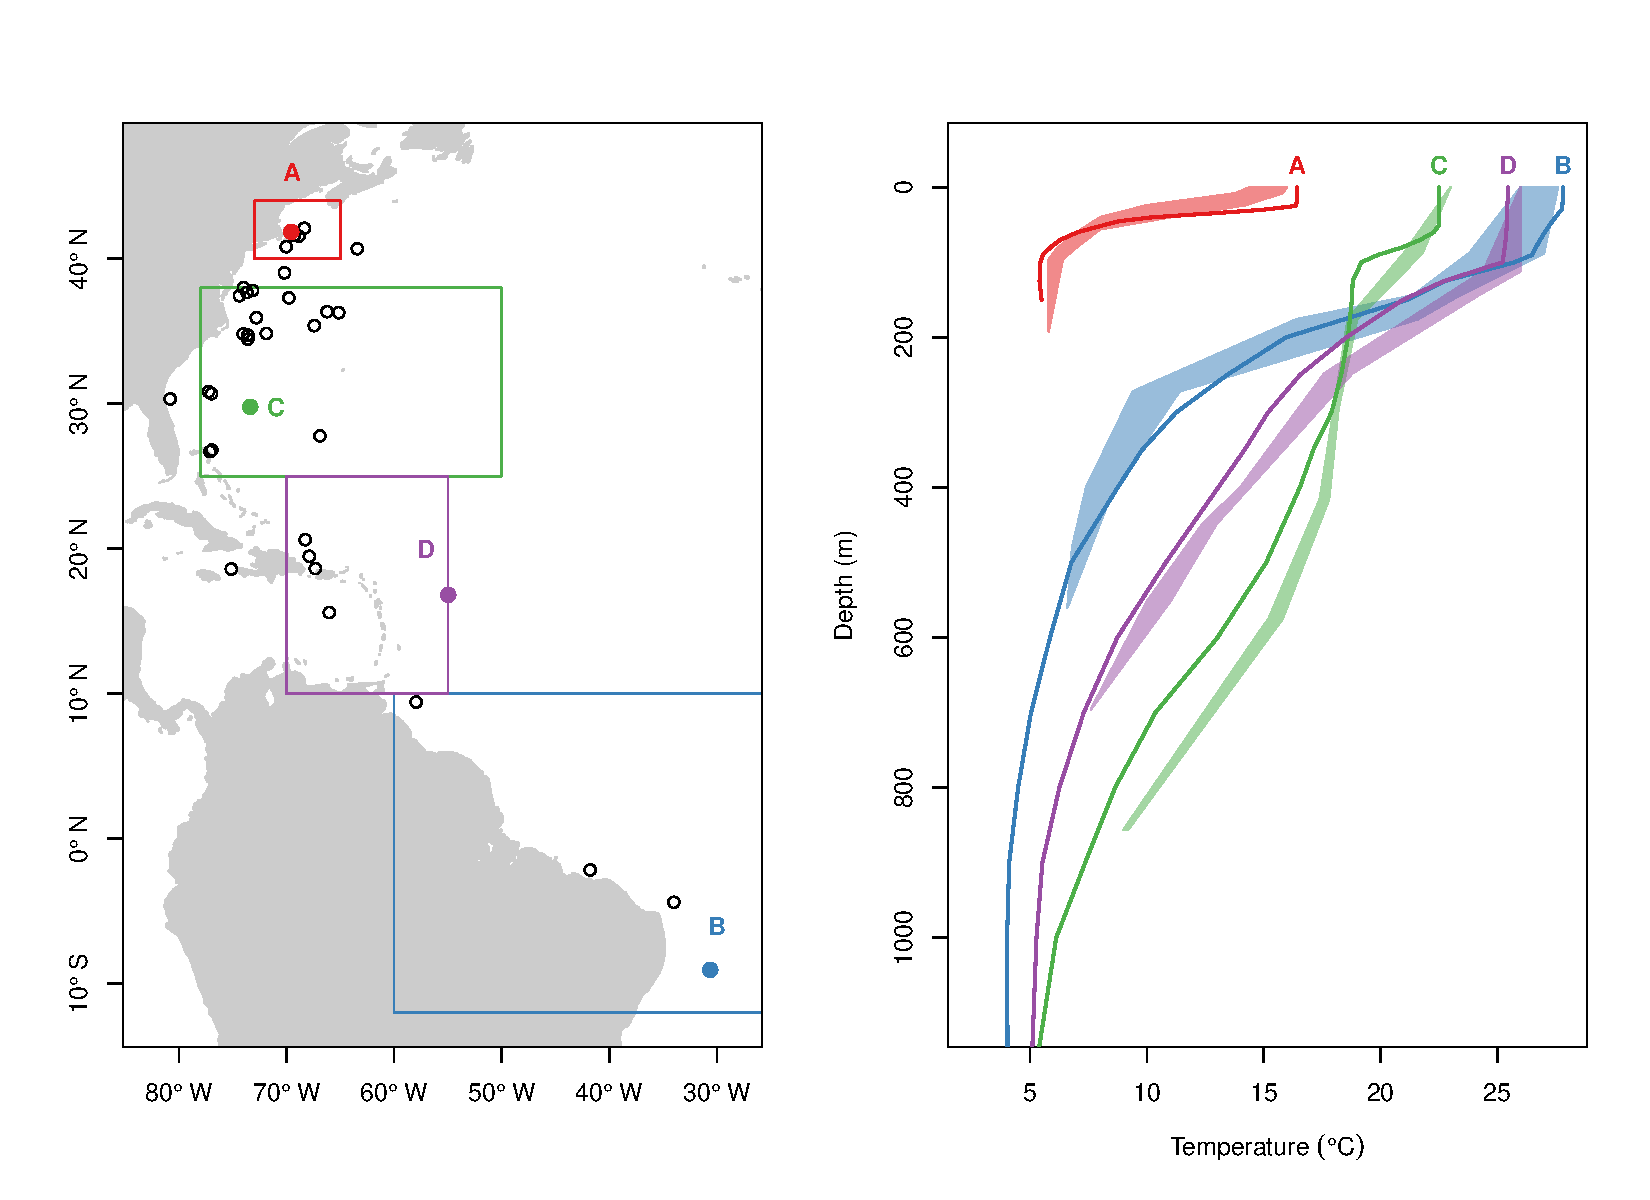
\includegraphics[width=1\textwidth]{images/C3_Fig1.pdf}
\caption[Comparison of depth-temperature profile data]{Example depth-temperature profile data from known pop-up locations of PSAT-tagged basking sharks. Selected, representative pop-up locations (color, left panel) from distinct regions of the study area were used to compare tag-based depth-temperature profiles (shaded from minimum to maximum recorded profile temperatures, right panel) to HYCOM profiles (lines, right panel) from the same time and location. Black circles (left panel) represent all tag pop-up locations in this study. Bounding boxes show the oceanographic regions discussed in the text, \cref{fig:c3f7} and \cref{tab:c3t2}.}
\label{fig:c3f1}
\end{figure}
%--------------------

\section{Results}
We tagged 57 basking sharks spanning sub-adult ($\sim$500-600 cm) and adult (> 600-700 cm) life stages (range 549-762 cm males, 549-823 cm females) and both sexes (10 females, 3 males, 31 unknown). Forty-five (79\%) of the 57 PSAT tags deployed between 2004-2011 reported. Eight tags released prematurely, and 1 of the tags had no useable data. Data from 37 of the remaining 44 tags contained sufficient information for further analysis (\cref{tab:c3t1}). These deployments averaged 234 days (SD 85 days, range 79-424 days). There was no evidence of tagging-induced mortality. Of the 35 tags that transmitted data (excluding two that were physically recovered), we received data representing 7\% (median, range 1-44\%), 26\% (median, range 4-61\%), and 52\% (median, range 7-91\%) of deployment days with light-based position estimates, SST, and depth-temperature profile data, respectively. The remaining two tags were physically recovered: one tag washed ashore in the Bahamas after 133 days at liberty and one was located on a beach in Rhode Island still attached to the deceased shark after a 78 day deployment. The full archival record was analyzed for these two deployments and contained light-based position estimates and SST data for 5-51\% and 66-89\% of deployment days, respectively, during which the animal occupied the surface (SST) or euphotic zone (light). Transmitted and archival profile data was available for more deployment days than either light-based position estimates or SST data in all but one of the reporting tags. One individual (B28) was tagged with a Fastloc GPS tag which reported 4 GPS snapshots over 3 days during winter (Dec. 22, 23, 26). These locations were fixed in the model runs for this individual, and no other usable GPS positions were acquired.

%--------------------
%Figure 2:
\begin{figure}[t!]
\centering
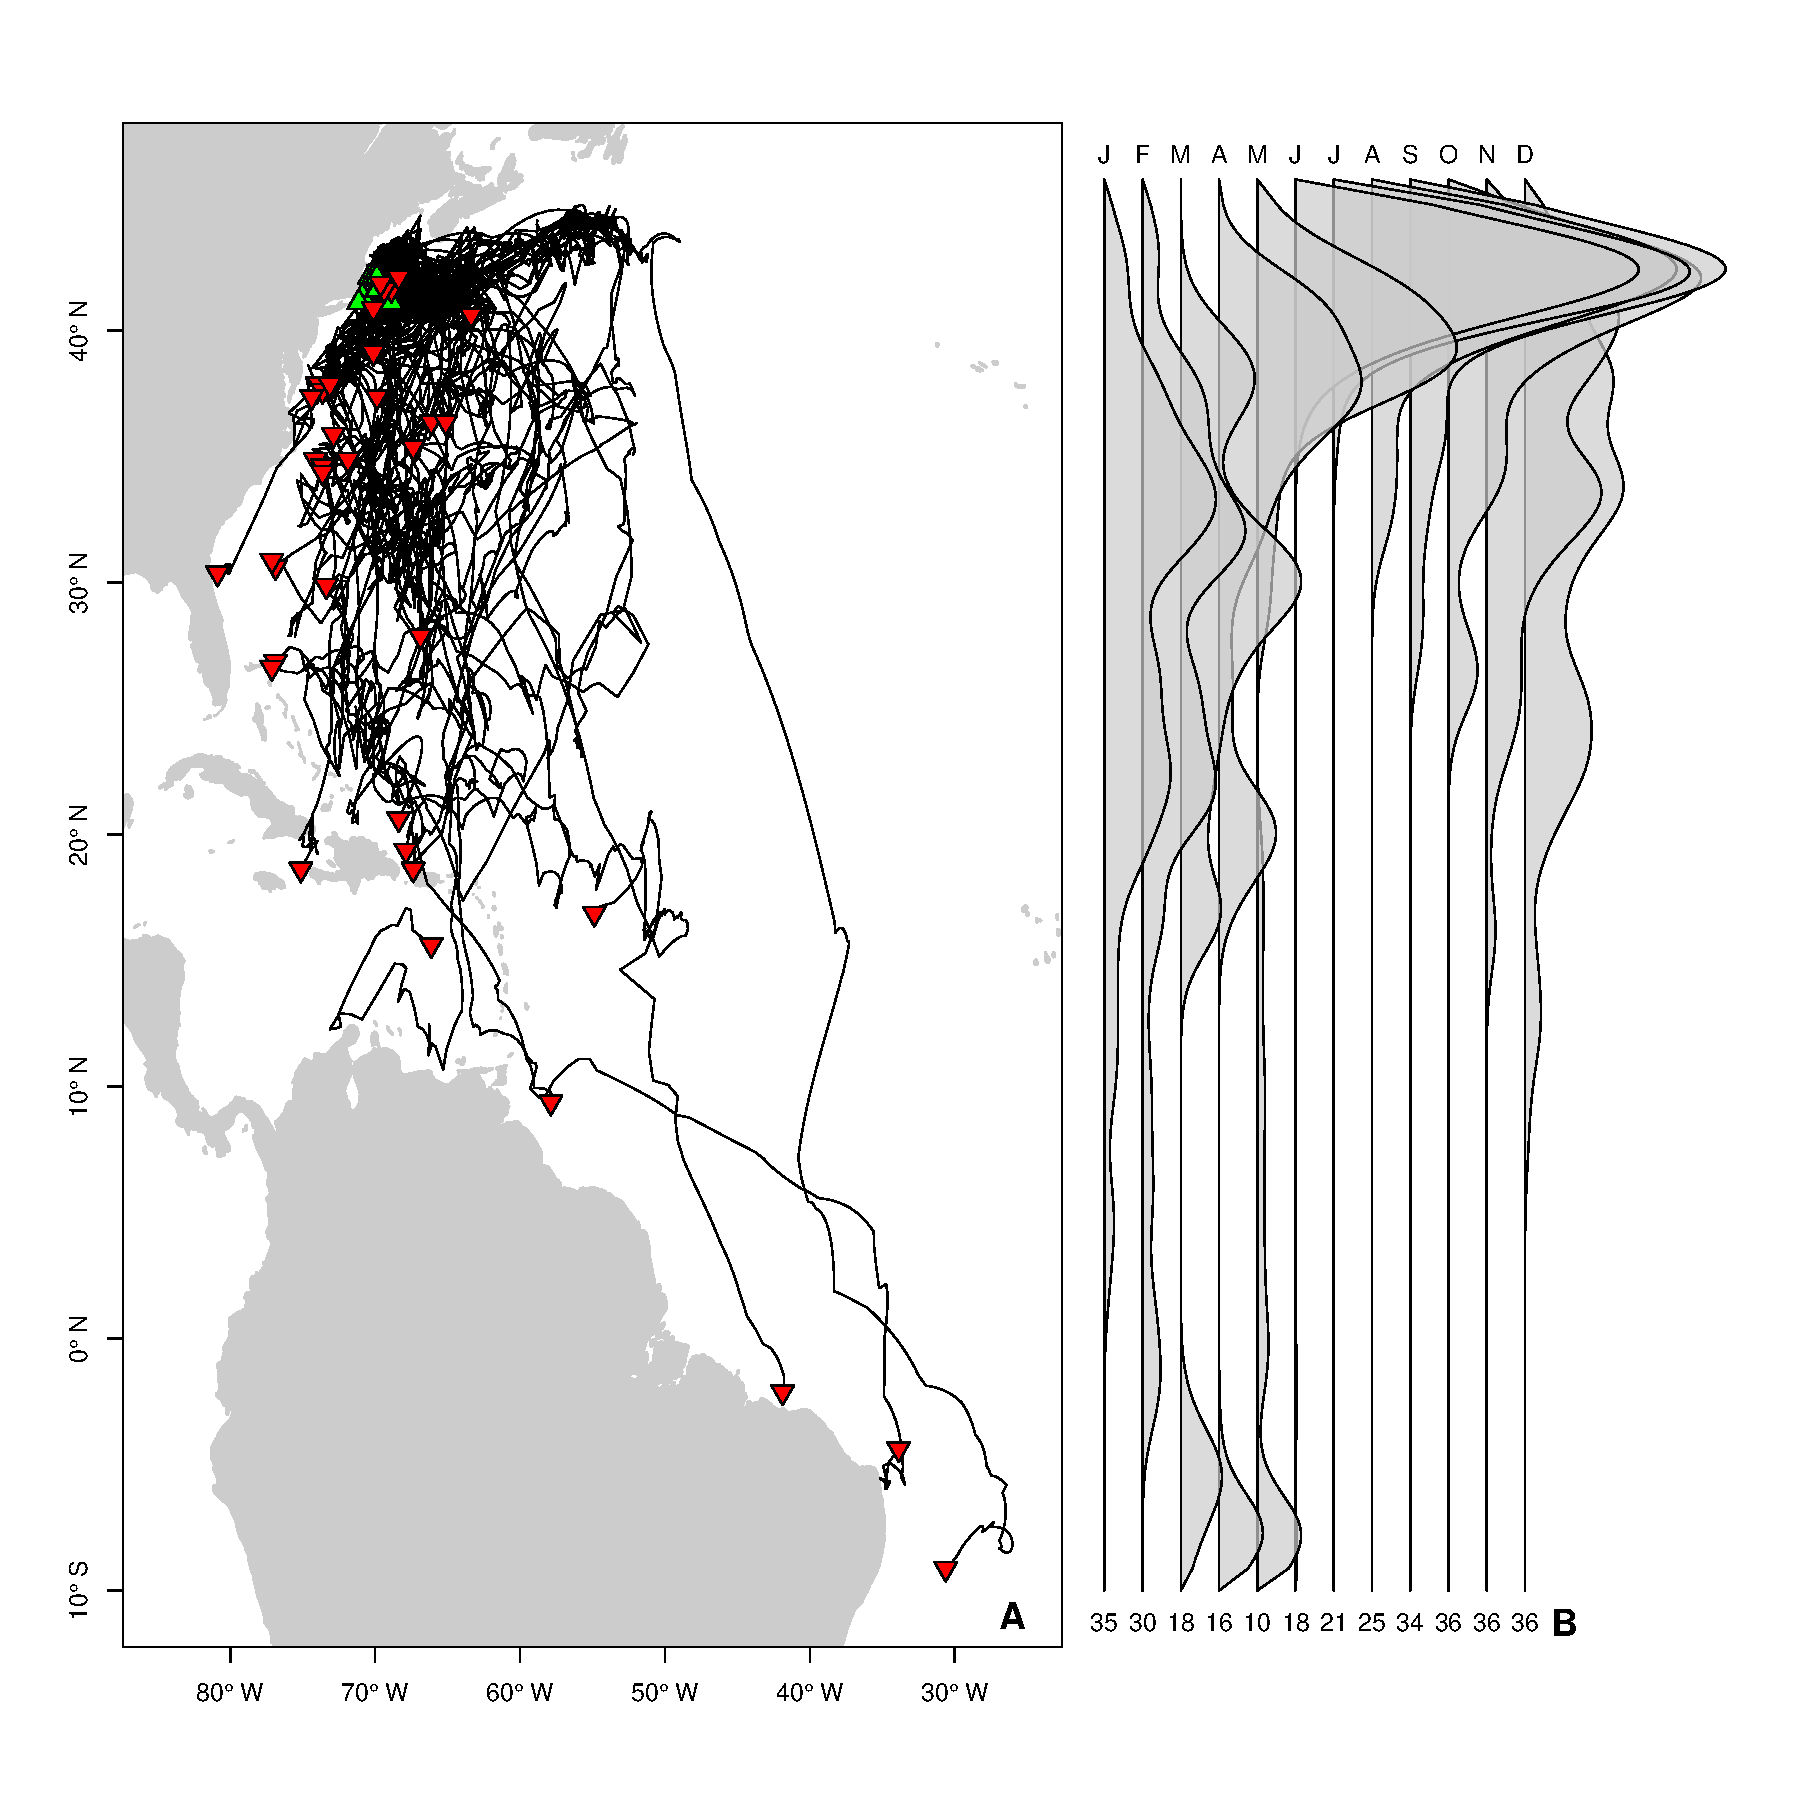
\includegraphics[width=.8\textwidth]{images/C3_Fig2.pdf}
\caption[Most probable basking shark tracks]{Most probable tracks (panel A) and latitude density by month (panel B) for 37 basking sharks satellite tagged off New England during June through October of 2004-2011. Tracks are plotted as black lines, and green and red triangles represent tag and pop-up locations, respectively. Letters above the density plot indicate month (\emph{e.g.} F=February), and numbers below indicate the number of individuals with tag data during that month.}
\label{fig:c3f2}
\end{figure}
%--------------------

For a given tag, varying amounts of each data type were obtained due to behavioral variability and individual differences in data transmission.  Model selection favored HYCOM-based profile likelihoods (\cref{fig:c3f1}) in 34 of 37 track calculations. Of the remaining 3 individual geolocation analyses, one favored OHC-based profile likelihoods, one WOA-based profile likelihoods and one model selection used only light and SST observations. Available light and SST data were not used in the selected model for 4 and 6 individual tag datasets, respectively (\cref{tab:c3t1}). Nearly all model outputs indicated the "migratory" behavior state was more likely once the tagged individual left the New England shelf (76\% of off-shelf position estimates), and this behavior remained dominant throughout the Sargasso Sea region (77\% of off-shelf position estimates). Shelf habitats near New England and from the Antillean Arc to the Amazon Delta were characterized by a higher likelihood ($\sim$50\% of on-shelf position estimates) of "resident" behavior (\eg slower, more tortuous movements).

While all tags were deployed off the northeastern coast of the U.S., most probable tracks showed a wide range of individual movements (\cref{fig:c3f2}). For individuals with sufficient data to perform the geolocation analysis (n=34), track distances ranged from 4009-17,387 km (mean 10,136 $\pm$ 3988 SD) spanning 79-424 days (mean 207 $\pm$ 107 SD). Several of the sharks showed relatively directed, long-range movements south from the tagging location in New England to the Puerto Rico Trench (n=4), Antillean Arc (n=3), and Amazon Delta (n=3) up to 17,387 km (6200 km displacement) from the tagging location (\cref{fig:c3f5}). Three individuals made transequatorial movements.

Movements of tracked sharks demonstrated strong seasonality (\cref{fig:c3f2}, \cref{fig:c3f3}) with individuals occupying coastal waters in high latitudes during the summer before moving south in fall (\cref{fig:c3f2}, \cref{fig:c3f3}), and all but one individual (B26) departed New England by January. This individual remained along the shelf edge between New England and the Grand Banks for the winter and returned to the New England canyons by late February (B26 in \cref{fig:c3f4}). All other tagged sharks overwintered in habitats as close as the Sargasso Sea and as far as the northeastern coast of Brazil before beginning to return to New England waters in late spring and early summer (\cref{fig:c3f2}, \cref{fig:c3f3}). Seven tags were deployed for > 300 days, including one for 423 days, and five of them transmitted sufficient data for track estimation. Six of these seven tags popped up in New England waters approximately one year after tagging, while the remaining tag reported near the Amazon Delta and represented the furthest southerly movements observed in this study (\cref{fig:c3f2}, \cref{fig:c3f5}). Eighteen tags exhibited deployment durations > 250 days, 10 of which (59\%) exhibited return migrations to the NWA, including one pop-up location 60 km from the tagging location one year later (B21). There was no significant difference in mean track distance between males and females (t-test, $p$=0.4633), although male sample size was low (n=3), and a linear regression analysis found no significant relation between shark size and extent of movement ($p$=0.27, $R^2$=0.05) or minimum latitude occupied ($p$=0.48, $R^2$=0.02).

Long-distance migrations often co-occurred with large vertical excursions and led to occupation of several distinct water masses throughout the year. Binned vertical histogram data (\cref{fig:c3f3}) were used to quantify where in the water column sharks tended to frequent. Overall, extensive vertical excursions characterized basking shark dive behavior when an individual left the continental shelf region of the eastern US (\cref{fig:c3f3}, \cref{fig:c3f4}, \cref{fig:c3f6}). Twenty-one individuals spent time below 1000 m, and it was likely that only limitations in earlier tag technology (maximum depth capability of 980 m) prevented those individuals' tags from recording similar behavior. The maximum depth recorded by a tag (shark B42) was 1504 m and recorded temperatures at depth in this study ranged from 4.2-29.9$^{\circ}$C. Recorded SST values from all individuals ranged from 7.4-29.9$^{\circ}$C (median 18.3$^{\circ}$C). Overall, 63\% of basking shark depth-temperature data was 8-18$^{\circ}$C, 87\% was between 6-20$^{\circ}$C, and all individuals made occasional forays into temperatures well outside those bounds (\cref{fig:c3f7}). In fact, one individual (B26) remained at northern latitudes (from Cape Cod to the Grand Banks) during winter and experienced < 10$^{\circ}$C ambient water temperatures for > 3 months (B26 in \cref{fig:c3f4}; range 4.8-12$^{\circ}$C from Nov 1 to Feb 15). 

Vertical habitat envelopes described the distinct water masses across the study area (from coastal New England to open ocean off Brazil), their depth-temperature characteristics, and the vertical behavior observed in each water mass (\cref{fig:c3f7}, \cref{tab:c3t2}). Generally, individuals spent much of their time in the epipelagic zone (< 200 m) during summer months at northern temperate latitudes where temperatures were typically < 20$^{\circ}$C (\cref{fig:c3f4}, \cref{fig:c3f6}, \cref{fig:c3f7}). However, during the fall, the majority of tagged individuals transitioned from the epipelagic orientation of the summer months to residency in the mesopelagic zone during the winter in which they cumulatively spent > 60\% of time between 400-1000 m (\cref{fig:c3f3}, \cref{fig:c3f4}, \cref{fig:c3f6}). Based on depth-temperature profile data, sharks remained below the euphotic zone for 27\% (median; range 0-90\%) of fall, winter and spring deployment days for which data existed, and this behavior exhibited no relationship with individual size or sex, although male sample size was low (n=3). Temperature profiles from these periods of mesopelagic occupation indicated this behavior occurred largely in the Sargasso Sea where warm (14-20$^{\circ}$C) water penetrates deep in the water column (profile C in \cref{fig:c3f1} and \cref{fig:c3f7}) resulting in relatively warm water at depth (\emph{e.g.} B20 and B22 in \cref{fig:c3f6} and \cref{fig:c3f7}). However, some sharks overwintered further south in the Guyana Basin and off the Brazilian shelf as indicated by warmer surface temperatures and a stronger temperature gradient with depth (\emph{e.g.} profile B in \cref{fig:c3f1}, B36 in \cref{fig:c3f6} and \cref{fig:c3f7}). Sharks generally inhabited warmer waters throughout winter at low latitudes, despite prolonged deep-water occupation, than the surface waters that they inhabited during summer months (\cref{fig:c3f7}, \cref{tab:c3t2}).

Shark B22 provided a good example of the distinct water masses traversed during a one-year deployment, with a complete round trip migration starting and ending in the tagging region (\cref{fig:c3f4}, \cref{fig:c3f5}). This individual occupied a well-mixed, cool surface layer in the Gulf of Maine during October before moving through the Gulf Stream and into the northern Sargasso Sea in November. This individual occupied the northern Sargasso from December to March before moving back into a more uniformly cool layer in April and May near Cape Hatteras. By June, both the estimated track and water characteristics indicate this individual had returned to the shelf-edge waters near New England and onto the shelf near Cape Cod by late September (\cref{fig:c3f4}).

%Figure 3:
\begin{figure}[t!]
\centering
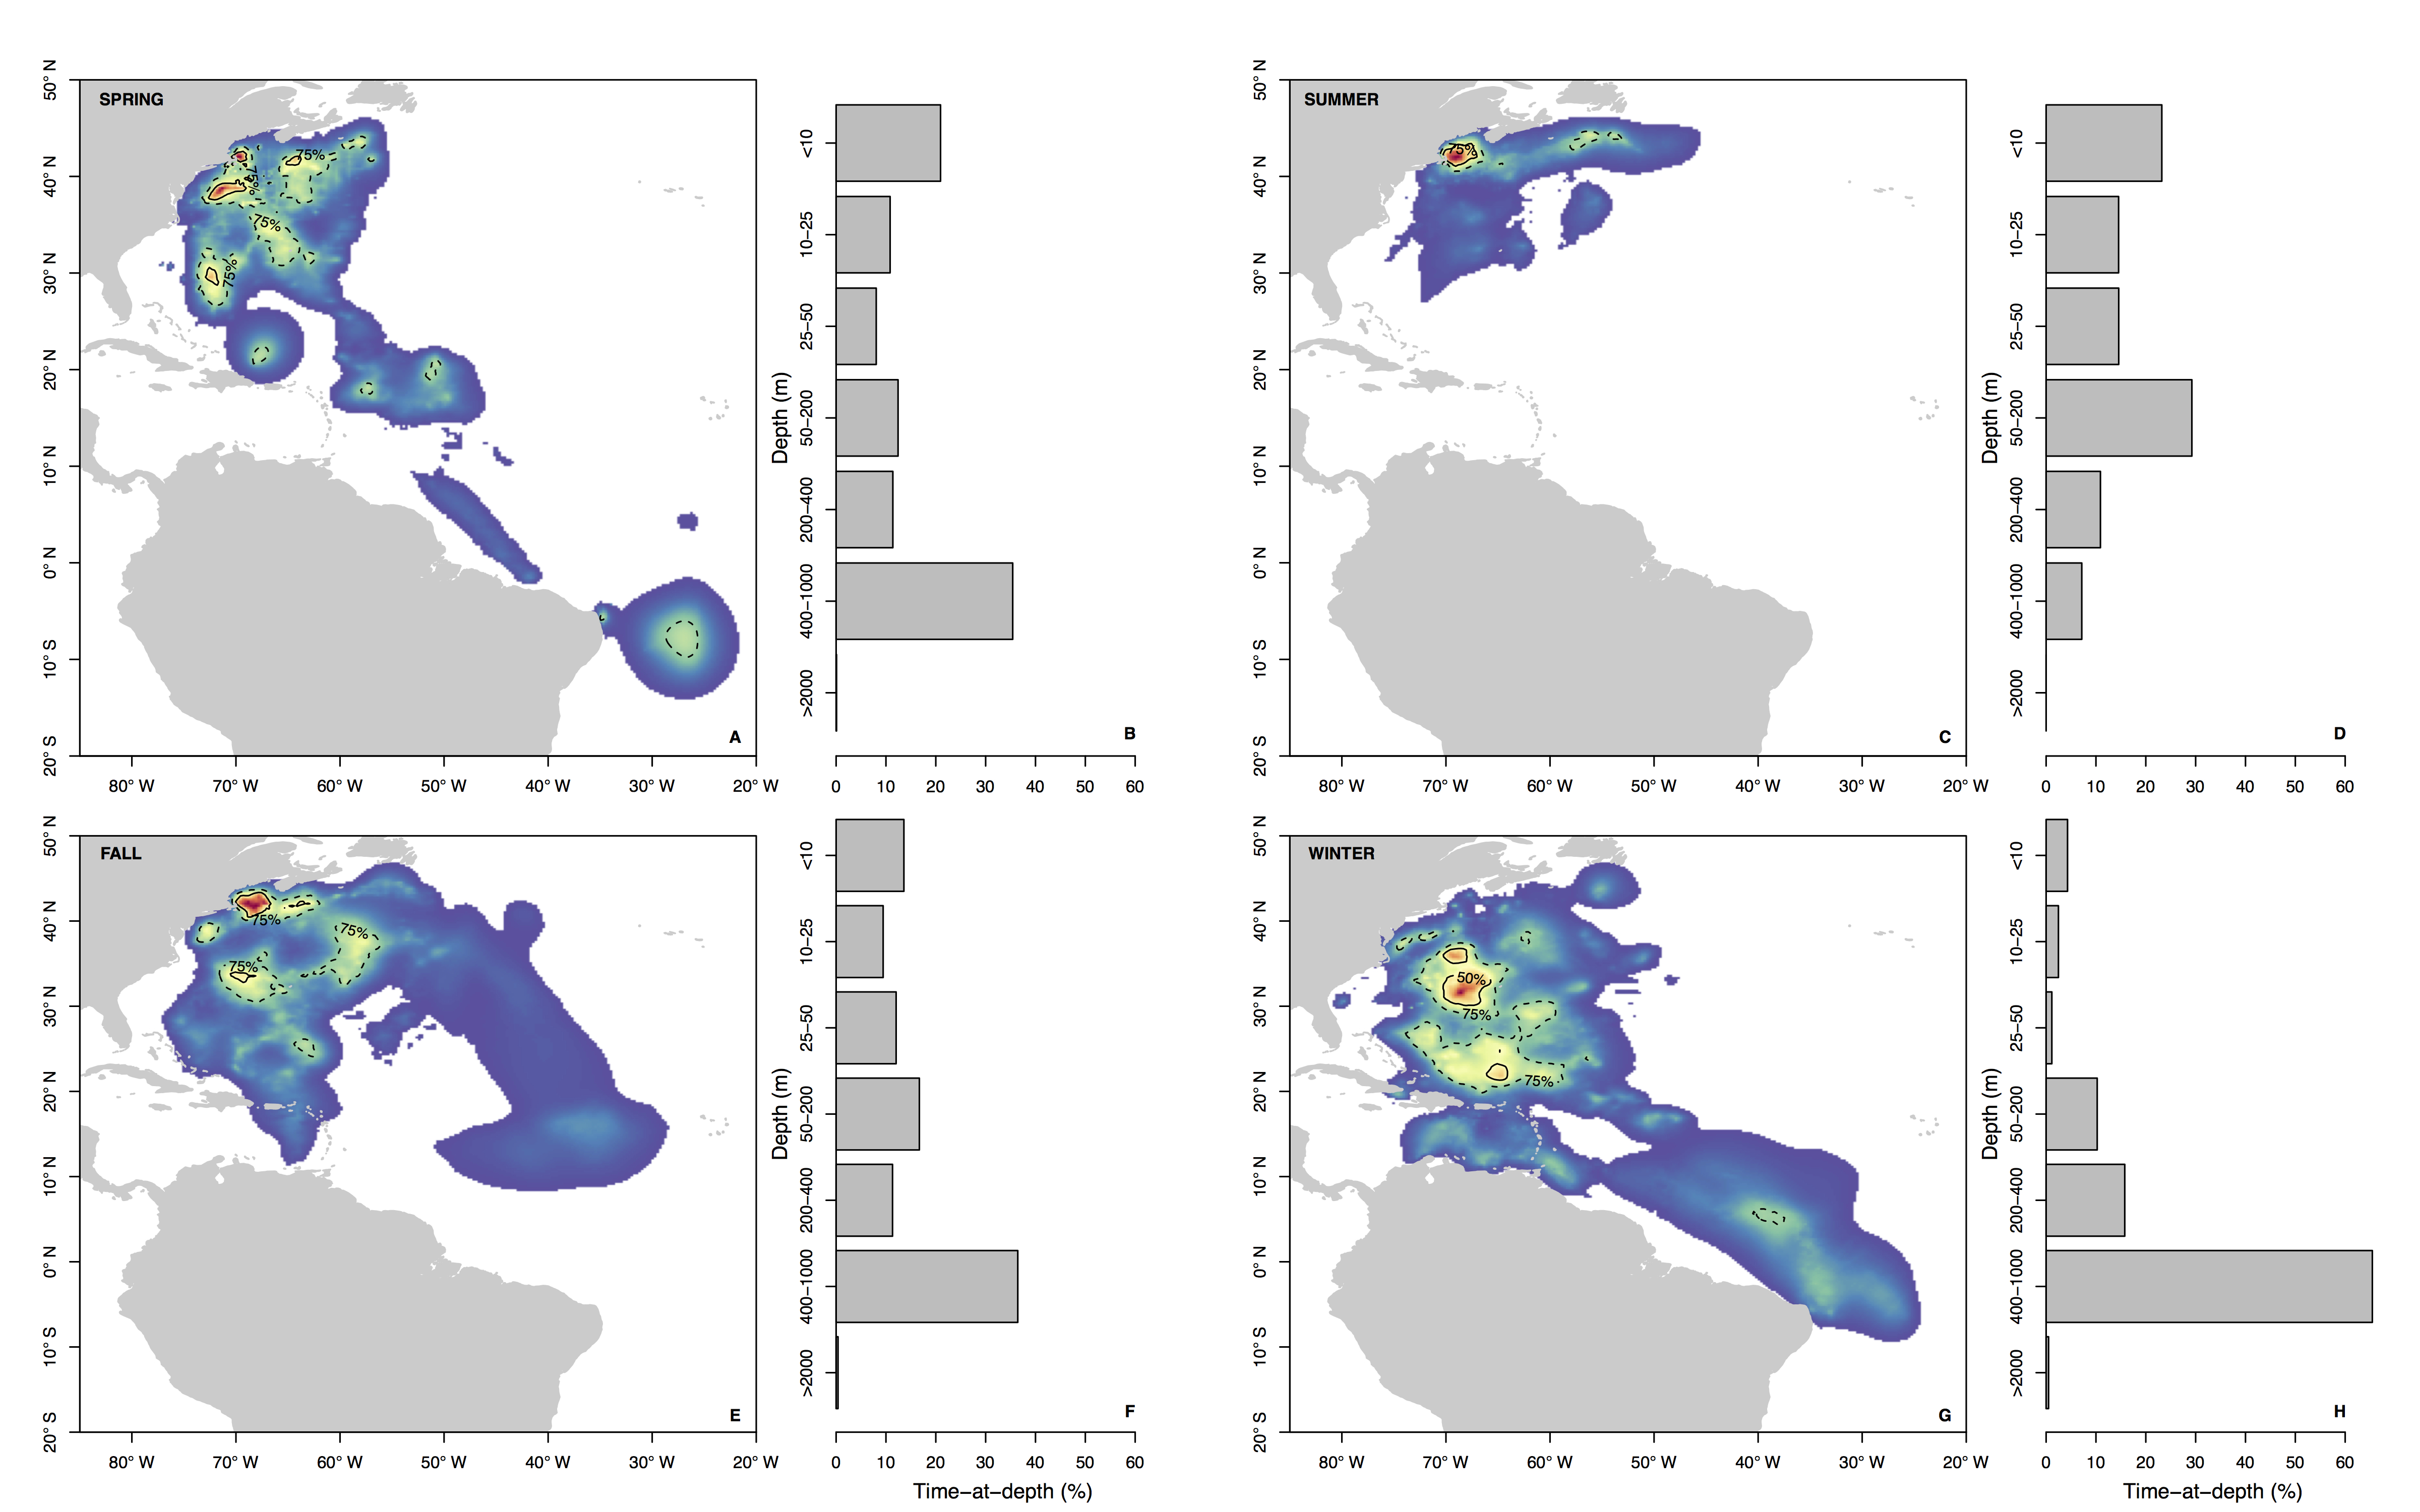
\includegraphics[width=1\textwidth]{images/C3_Fig3.jpg}
\caption[Basking shark seasonal residency distributions]{Seasonal residency distributions (panels A, C, E, G) and cumulative time-at-depth (panels B, D, F, H) for spring (A, B), summer (C, D), fall (E, F), and winter (G, H). Residency distributions were calculated using the \texttt{HMMoce} package for \texttt{R}. Contour lines represent 50\% and 75\% of occupation for a given season as depicted by solid and dashed contours, respectively. }
\label{fig:c3f3}
\end{figure}

%Figure 4:
\begin{figure}[t!]
\centering
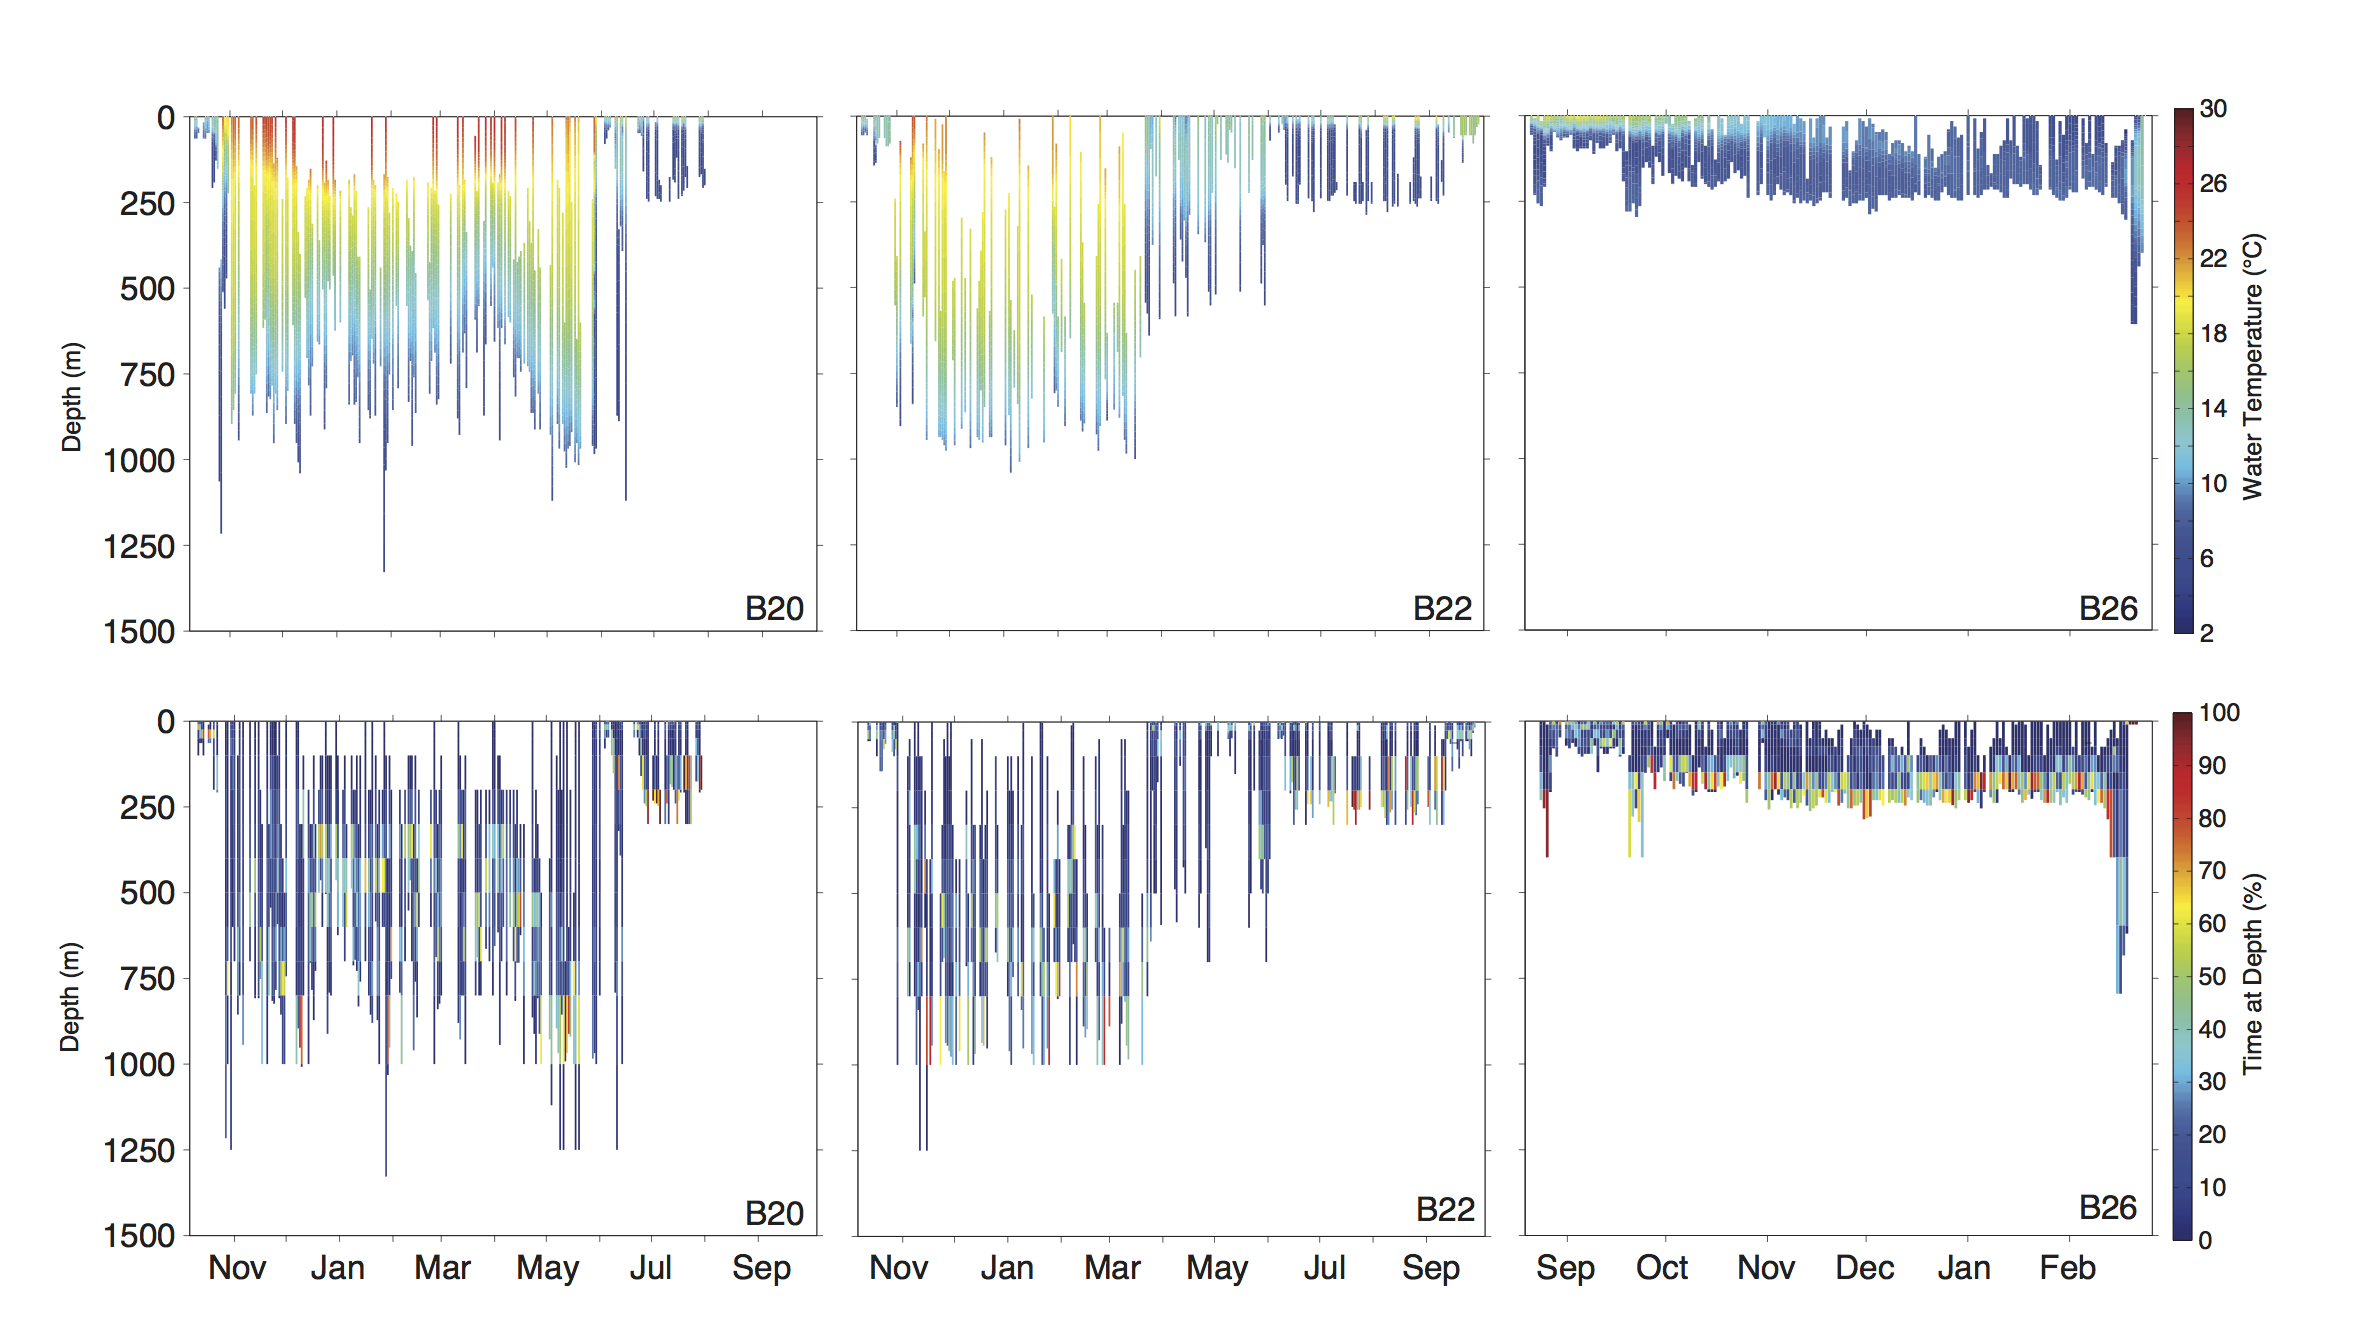
\includegraphics[width=1\textwidth]{images/C3_Fig4.jpg}
\caption[Representative basking shark vertical data]{Daily depth-temperature profiles (row 1) and time-at-depth profiles (row 2) for 3 representative basking sharks (tracks plotted in \cref{fig:c3f5}A). Note differing time scale (x-axis) among individuals.}
\label{fig:c3f4}
\end{figure}

%Figure 5:
\begin{figure}[t!]
\centering
\includegraphics[width=1\textwidth]{images/C3_Fig5.jpg}
\caption[Example long-range basking shark movements]{Movements of selected individuals demonstrating representative behaviors exhibited by sharks in this study. Two selected individuals exhibited site fidelity to Cape Cod (B20, B22) and one individual overwintered near Newfoundland (B26, panel A). The variety of long distance movements are represented by three individuals with pop-up locations from the eastern Caribbean to the SE coast of Brazil (panel B). Tracks are plotted as points colored by month, and green and red triangles represent tag and pop-up locations, respectively. Text labels correspond to Shark ID in \cref{tab:c3t1}, and blue background indicates bathymetry of the region. Vertical habitat use of these selected individuals is shown in \cref{fig:c3f4} and \cref{fig:c3f6}. }
\label{fig:c3f5}
\end{figure}

%Figure 6:
\begin{figure}[t!]
\centering
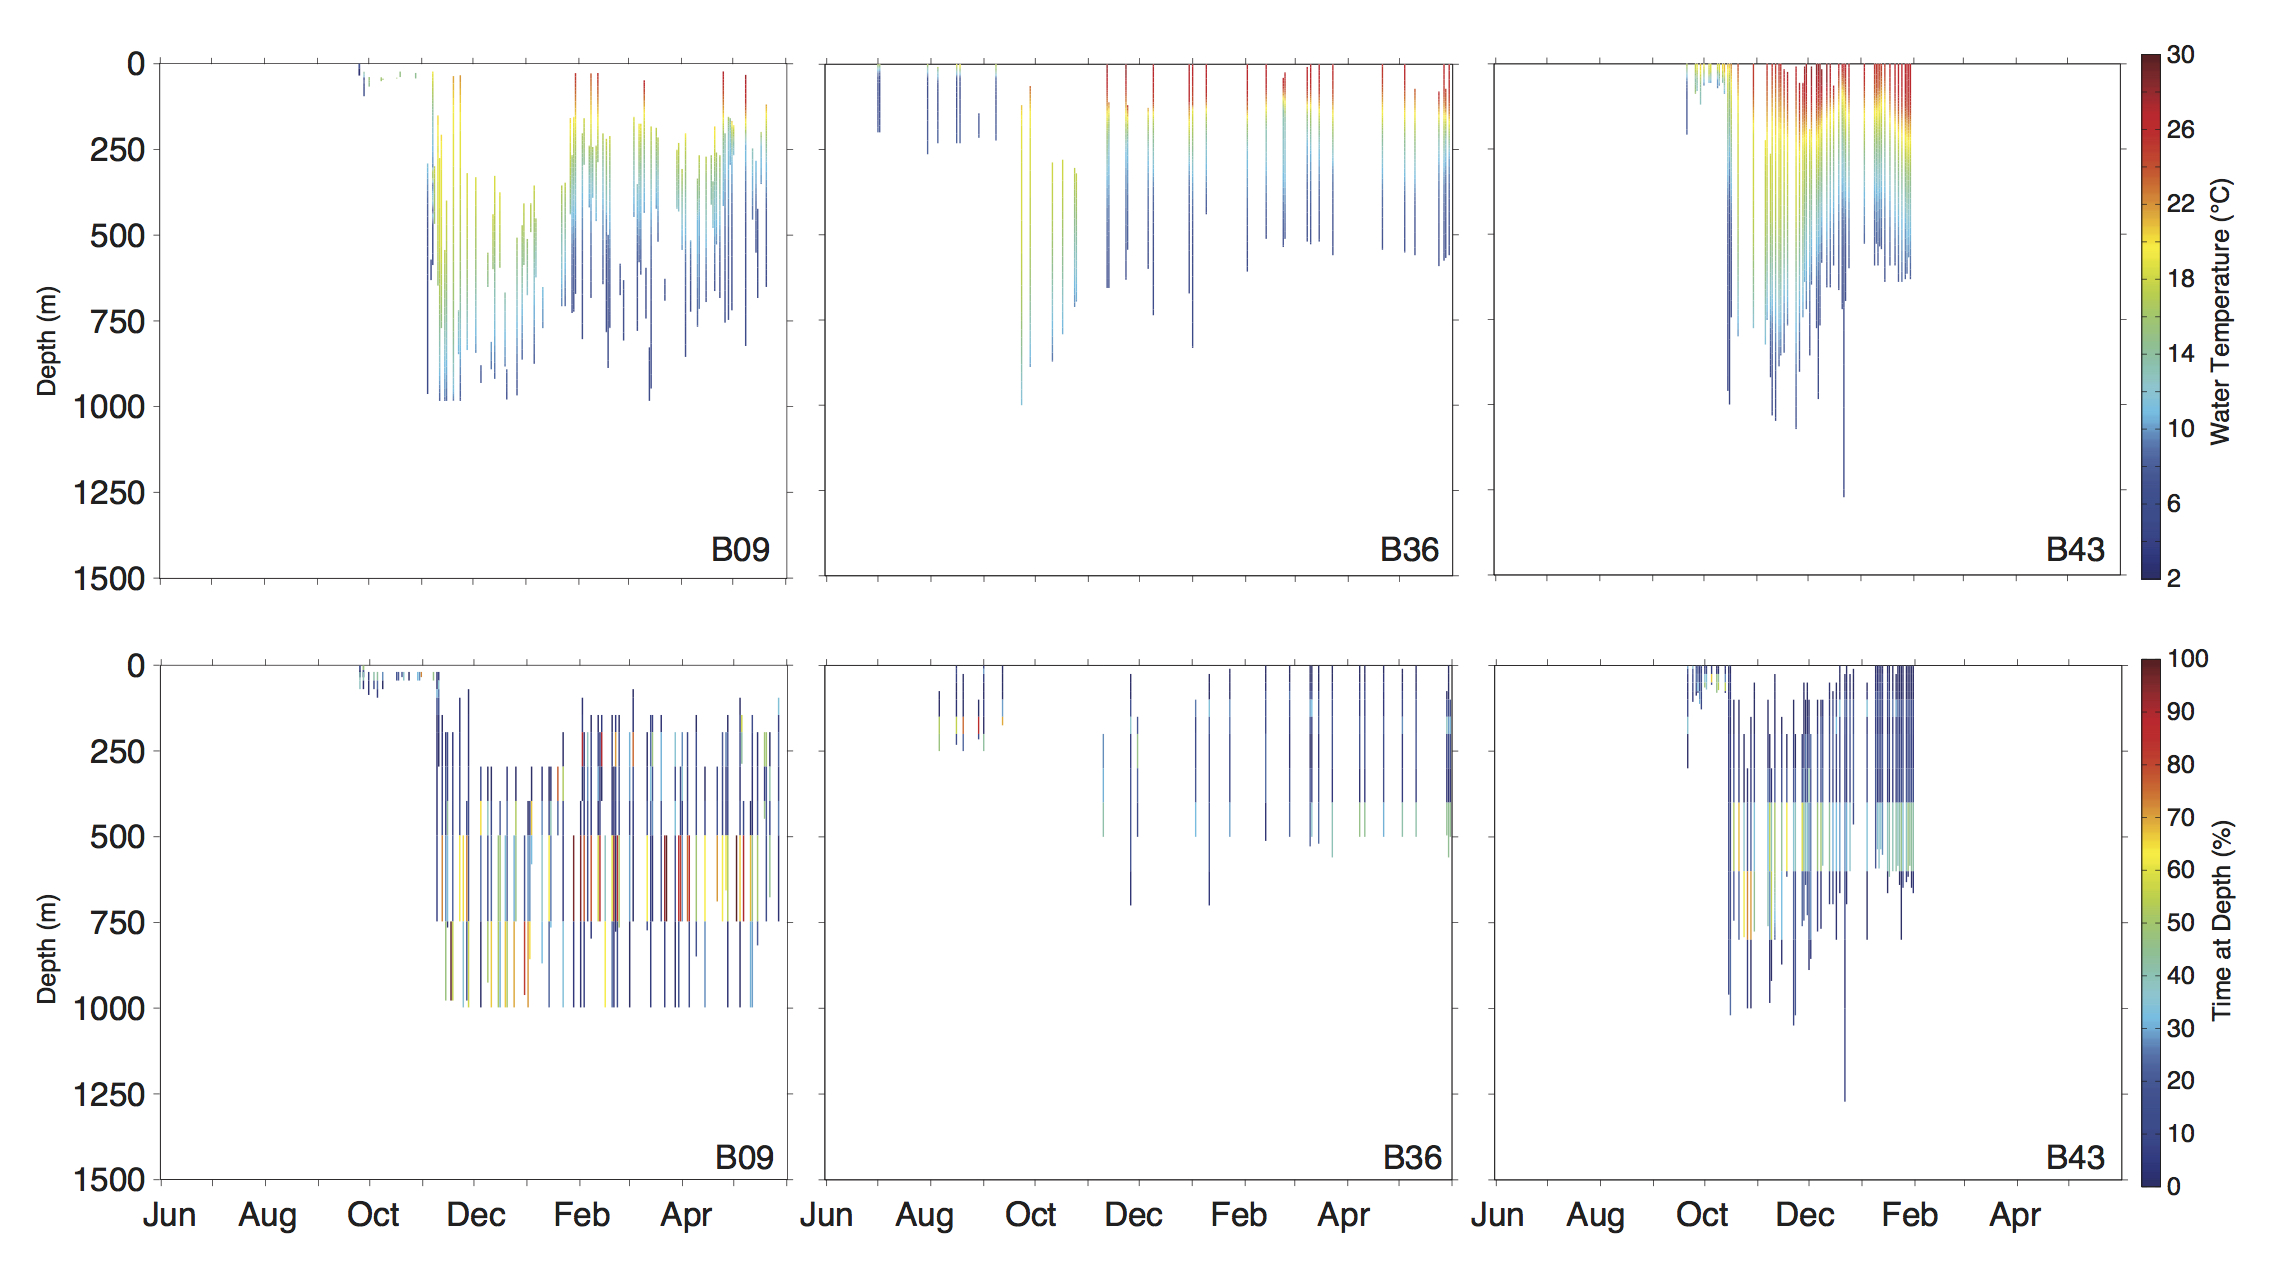
\includegraphics[width=1\textwidth]{images/C3_Fig6.jpg}
\caption[Representative basking shark vertical data for long-range movements]{Daily depth-temperature profiles (row 1) and time-at-depth profiles (row 2) for 3 representative basking sharks (tracks plotted in \cref{fig:c3f5}B). Note differing time scales (x-axis) among individuals.}
\label{fig:c3f6}
\end{figure}

%Figure 7:
\begin{figure}[t!]
\centering
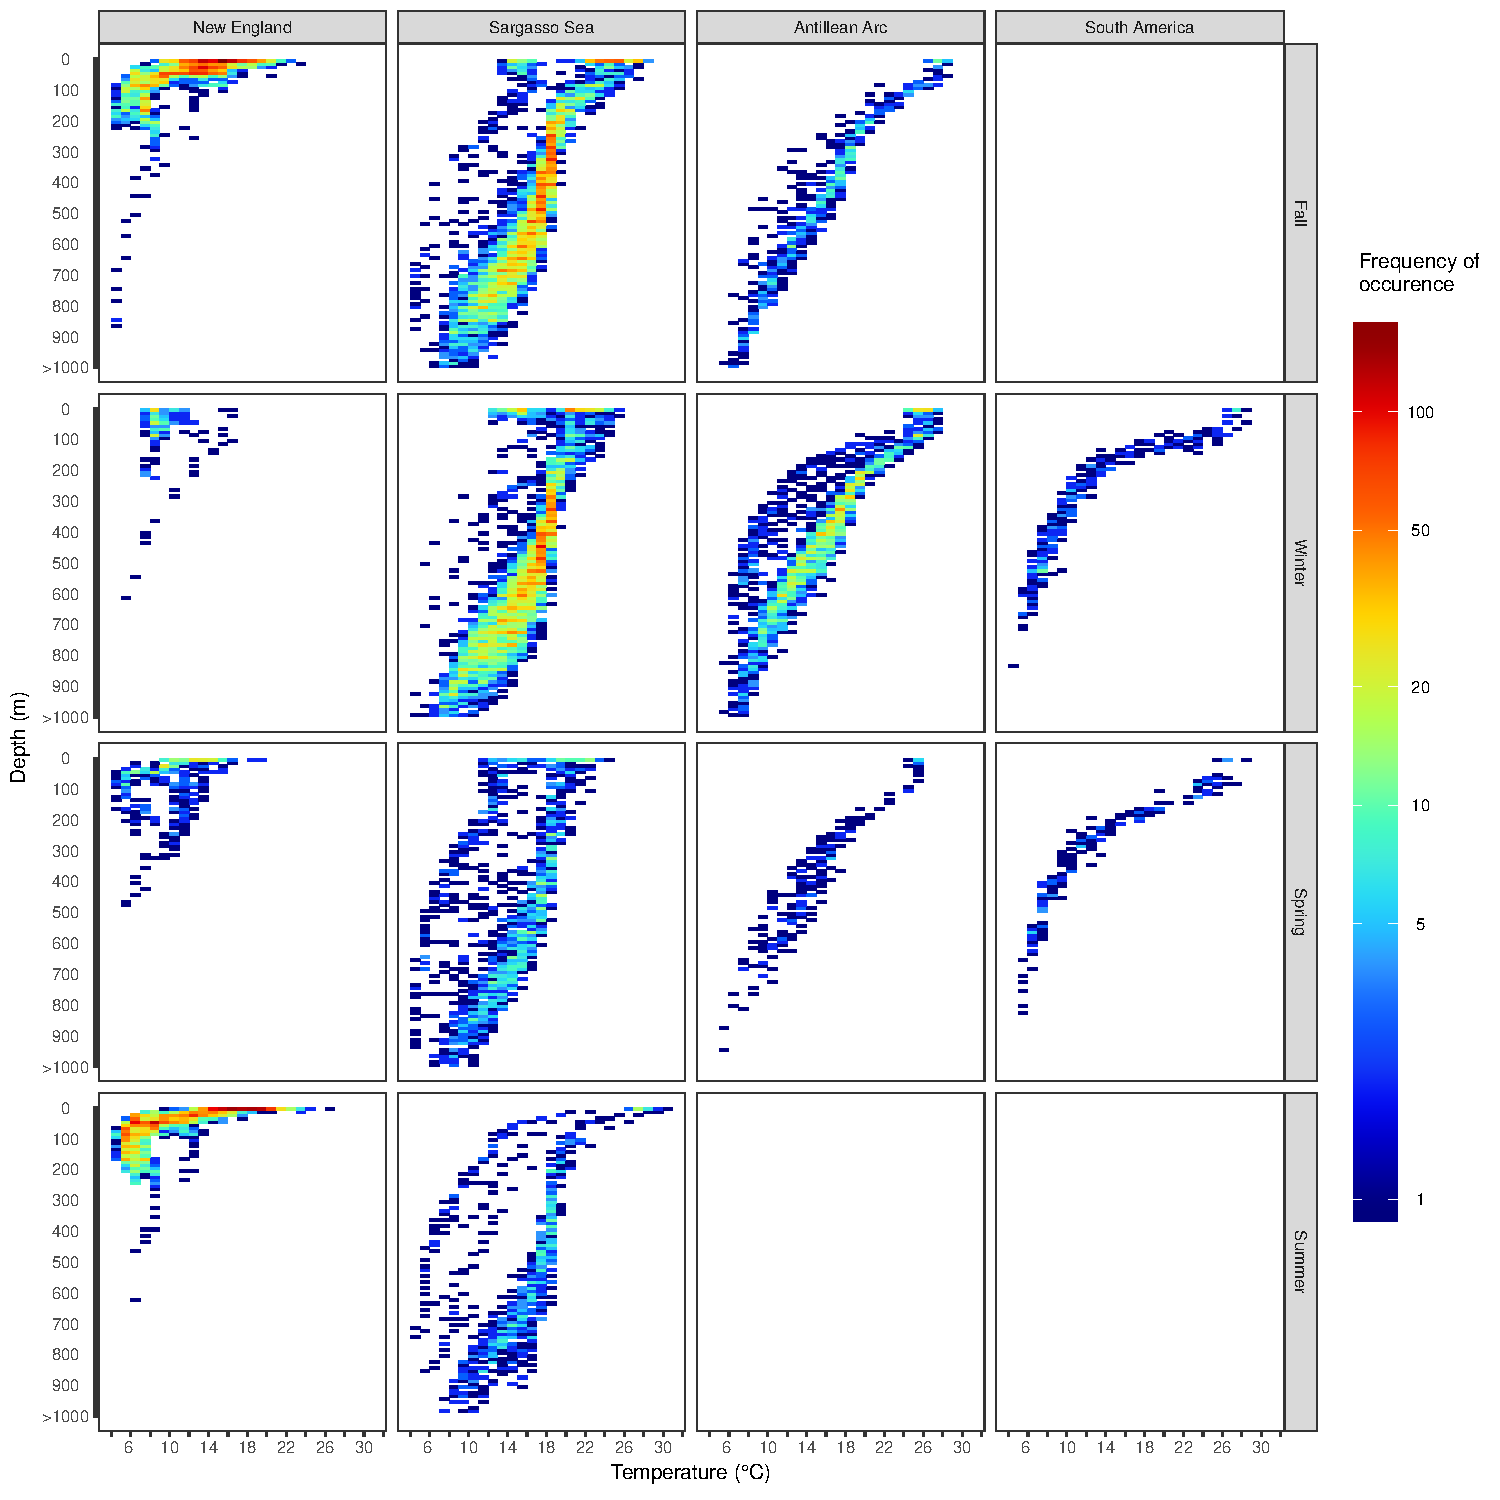
\includegraphics[width=1\textwidth]{images/C3_Fig7.pdf}
\caption[Basking shark vertical habitat envelopes by season]{Vertical habitat envelopes of basking sharks. Temperature and depth data are binned every 1$^{\circ}$ and 25 m, respectively. Depths deeper than 1000 m are added to the last bin. The bounds for each region are shown as boxes in \cref{fig:c3f1}. Note the color bar is on a log scale. Summary statistics for each region and season are shown in \cref{tab:c3t2}, and blank panels indicate no data was collected for that region-season combination. }
\label{fig:c3f7}
\end{figure}

\section{Discussion}
It is increasingly clear that pelagic fishes throughout the global ocean conduct long-range migratory movements \citep[\emph{e.g. }][]{Block2011,Skomal2017a} and connect the surface and deep ocean through meso- and bathypelagic dive behavior \citep{Braun2014,Thorrold2014a}. The basking sharks tagged in the present study were no exception, making some of the longest horizontal movements of any ocean species tagged to date \citep{Block2005,Bonfil2005,Hays2006,Skomal2017a}.  Tagged individuals moved through several distinct water masses of the western Atlantic, and spent significant time in the mesopelagic, demonstrating the ability of basking sharks to traverse a wide range of environments from the surface to deep ocean across a 25$^{\circ}$C temperature range.

Movements through distinct water masses often coincided with varying periods of deep water occupation. Nearly all tagged individuals demonstrated a shift to residency from surface waters to deep in the meso- and bathypelagic during colder months that may explain the apparent disappearance of basking sharks during winter \citep{Parker1954}. While our results corroborate previous studies that suggest seasonally variable dive behavior \citep{Sims2003} and southward migration during winter \citep{Doherty2017}, sharks in this study made much more extensive movements throughout the open ocean than those observed in similar studies elsewhere \citep{Doherty2017} and spent up to several months at mesopelagic depths. Sharks tagged in the northeast Atlantic (NEA) did make dives to similar maximum depths ($\sim$50\% of tagged individuals dove below 1000 m; \citealt{Doherty2017}) but averaged > 80\% of time above 200 m and < 10\% deeper than 500 m \citep{Sims2003, Doherty2017}. The mesopelagic occupation observed in this study suggests this behavior is much more ubiquitous among NWA basking sharks as they move throughout the open ocean than their NEA conspecifics that are relatively close to the coast and may be a product of the oceanography experienced (\emph{e.g.} warm, homogenous depth-temperature profiles in the Sargasso Sea) by these individuals in the open ocean of the NWA. 

The other main difference in behavior among these regions is the winter migration strategy. NEA basking sharks moved south from Ireland and the UK to the Bay of Biscay, but despite tagging 70 basking sharks with satellite tags, only 1 individual traversed > 20$^{\circ}$ of latitude after summer occupation of the far northern latitudes \citep{Doherty2017}. In contrast, winter movements at and beyond this scale were more commonly observed in the NWA \citep[][ and this study]{Skomal2009}. These movements refute the suggestion that basking sharks are largely restricted to temperate latitudes \citep{Sims1999,Sims2003,Gore2008,Doherty2017}, while NEA basking sharks did not traverse the equator, movements by individuals in the NWA demonstrate that tropical environments do not pose a barrier to basking shark movements.

It seems likely that the long-distance movements by basking sharks that we documented are driven, at least in part, by the dynamic oceanic environment of the western Atlantic Ocean. The NWA is punctuated by strong seasonal fluxes in pelagic primary productivity \citep{Miller2012} and temperature \citep{Talley2011}. The warm water and high productivity attract many species to the temperate NWA during summer (\emph{e.g.} basking sharks, \citealt{Curtis2014}; white sharks, \citealt{Skomal2017a}). While it is clear basking sharks are able to tolerate sub-10$^{\circ}$C water for months at a time (B26 in \cref{fig:c3f4}; \citealt{Sims2008}), individuals in this study spent much of their time overwintering in warm, mesopelagic waters. In fact, as a whole, sharks spent more time in warmer water during deep occupation periods in winter as they moved south than they did during summer. While the function of this deep occupation is unknown, the Sargasso Sea is a relatively stable, warm water mass during winter months and may host prey opportunities for basking sharks in the mesopelagic, including a substantial deep scattering layer that overlaps with basking shark depth use (400-600 m; \citealt{Irigoien2014}) and potentially co-occurring anguillid eel spawning aggregations \citep{Wysujack2015}. These migrations away from the northern winter may also be associated with hotspots of relatively high production at lower latitudes \citep[\emph{e.g.} Brazilian shelf; ][]{Mourato2014}. Movements in this study demonstrated orientation to shelf edge habitats, particularly along the northern coast of Brazil during winter, that likely host persistent fronts \citep{LeFevre1987,Sims2008} and thus relatively high primary production even at low latitude. While basking sharks have been shown to orient to persistent seasonal fronts \citep{Miller2015}, most individual tracks in this study demonstrated intense occupation of near-shelf regions that was punctuated by lengthy offshore excursions. Thus, perhaps the combination of favorable growth energetics associated with warm overwintering habitat (relative to overwintering at temperate latitudes) and food availability drive southerly movements away from temperate latitudes for winter and the mesopelagic occupation in (sub)tropical waters observed here. However, further work is needed to test the role of energetics and food resources as drivers of basking shark migrations.

Movement patterns of tagged basking sharks may also be associated with reproduction \citep{Skomal2009}. Basking sharks are commonly observed along the northeastern US during summer, presumably to forage; however, mating may also occur during this period while sharks are aggregated and potential courtship behavior has been observed \citep{Wilson2004a}. Subsequent movements into the tropical Atlantic and occupation of mesopelagic depths may be a predator avoidance or parturition strategy as these environments are characterized by mild, stable conditions. This may further explain the lack of observations of pregnant females despite prolonged coastal fisheries in the NEA \citep{Sims2008}. Thus, while we did not observe significant differences in movement between sexes, the females that undertake long-range southerly migrations may be exploiting stable environmental conditions for gestation and parturition, and the stable habitat and relative lack of predators may provide suitable nursery habitat for neonates. The presence of < 2.5 m TL basking sharks in the Gulf of Mexico during spring \citep{Hoffmayer2011} lends some support for this hypothesis as it suggests that parturition is occurring during winter months in tropical or subtropical waters. The wide variation in movement patterns (> 50$^{\circ}$ range in latitude) suggests these migrations were not driven by a localized mating event somewhere in the Atlantic. Unfortunately, we were unable to sex a significant portion of tagged individuals in this study due to tag application methods, and the limited sample size of sexed individuals indicates no difference in movements between sexes that may further clarify reproductive hypotheses. 

Highly variable dive behavior, including extended forays away from the photic zone, exhibited by basking sharks made traditional light-based geolocation difficult in our study. Thus, we employed a recent advance \citep[based on extensive work by ][]{Pedersen2008, Pedersen2011a} in geolocation analysis methods to supplement missing light data with other forms of data recorded on the tag \citep{Braun2018a}. Depth-temperature profiles, in particular, provided substantially more information to be used for geolocation than light and SST data used in traditional geolocation approaches. These profiles provided observations that were used for geolocation when tagged individuals were away from the surface and the tags couldn't collect light and SST metrics. In addition, the profile data yielded diagnostic depth-temperature profiles that can be compared to modeled or in situ oceanographic data for reducing geolocation error \citep{Braun2018a}. By using the high-resolution (0.08$^{\circ}$) HYCOM reanalysis product, we were able to leverage the synoptic daily coverage of an oceanographic model that incorporates available in situ data to improve geolocation estimates. While previous tracking studies have shown some problems with the HYCOM reanalysis product being used to construct tracks through the Gulf Stream eddy field \citep{Braun2018a}, the majority of basking sharks in this study moved latitudinally and spent relatively little time in the most dynamic regions of the NWA. 

Model outputs also indicated a higher likelihood of "resident-like" movements in productive shelf habitats around New England and off the Antilles and South America. It is likely these restricted movements are indicative of foraging in these relatively productive shelf habitats \citep{Mourato2014}. In contrast, migratory movements (4 $m \cdot s^{-1}$) were more likely in pelagic waters, including during overwintering in the Sargasso Sea. Because of model formulation, the higher speeds that we classified as "migratory" may also be more likely, overall, due to the scale at which the observation likelihoods are formulated. For instance, if tag-based SST corresponds to remotely sensed SST over a broad area (\emph{e.g.} Sargasso Sea), we may expect migratory behavior to be more likely than the resident behavior that would result from more constrained likelihoods (\emph{e.g.} tag-based SST matching more closely to a confined region). While this approach is significantly more computationally-intensive than traditional light-based geolocation approaches, comparing tag data directly to in situ and/or modeled oceanographic profiles from the same time frame results in a more realistic representation of shark movements and the oceanographic environment they inhabit.

The basking shark tracks documented here represent the largest scale movements reported for basking sharks, including one individual's estimated track distance covering >17,000 km, and the deepest dive recorded by a basking shark (1504 m). The observed tracks further expand the known range of basking sharks reported by \citet{Skomal2009}. We recorded 3 individuals making transequatorial migrations yet no tagged individuals made significant longitudinal movements toward the NEA. North-south movements were, therefore, much more common in the portion of the NWA population sampled here than east-west movements that may, in turn, limit the exchange of genetic material between the NWA and NEA. In contrast, \citet{Gore2008} found that one of two satellite-tagged basking sharks moved from the Isle of Man to the eastern coast of Newfoundland in less than 3 months. In addition, there is little evidence for genetic structuring of basking sharks in the Atlantic \citet{Hoelzel2006}, suggesting sufficient connectivity to at least maintain panmixia between NEA and NWA populations.

\section{Conclusion}
The current reliance on light levels for geolocation of many marine fishes renders geolocation impossible when tagged individuals spend significant time below the euphotic zone. Tagged sharks in this study spent significant time at mesopelagic depths, particularly during winter, at which light levels were too low for geolocation. We supplemented light-based geolocation with position estimates generated by matching depth-temperature profiles collected by the sharks' tags to in situ or modeled oceanographic profiles. Our approach provided considerably more information on movement patterns than are typically available from PSAT data with limited light-level information, providing a valuable method for studying marine species that do not frequent the euphotic zone. The resulting basking shark tracks demonstrated large-scale movements up to over 17,000 km from Cape Cod to southern Brazil, winter residency in New England waters, and a range of behaviors in between. Most individuals exhibited seasonal movements into the Sargasso Sea during winter and multiple deployments of sufficient duration captured the return migration to Cape Cod the subsequent summer. Basking sharks in this study traversed multiple distinct water masses through the western Atlantic and exhibited basin-scale movements that warrant international cooperation for adequate management of this species. Winter habitat use was characterized by occupation of mesopelagic waters at low latitudes during which individuals often left the surface for months at a time. This cryptic deep-water overwintering provides impetus for further study of this poorly understood species.


%--------------------
%\begin{landscape}
% table 1: tag metadata and results
\begin{table}[t!]
\caption{Summary information from satellite tag deployments on \textit{Cetorhinus maximus} in the NW Atlantic.}
\label{tab:c3t1}
\centering
\scriptsize
%\begin{tabular}[t]{lrllrlll}
\begin{tabular}{p{.75cm} p{.85cm} p{1.5cm} p{.5cm} p{.5cm} p{.75cm} p{.75cm} p{.5cm} p{.75cm} p{.75cm} p{.5cm} p{.5cm} p{.5cm} p{.5cm}}
\toprule
\textbf{Shark ID} & \textbf{Tag Type} & \textbf{Tag Date} & \textbf{TL (m)} & \textbf{Sex} & \textbf{Pop Lat ($^{\circ}$N)} & \textbf{Pop Lon ($^{\circ}$W)} & \textbf{TAL (d)} & \textbf{Depth (m)} & \textbf{Dist. (km)} & \textbf{Light (\%)} & \textbf{SST (\%)} & \textbf{PDT (\%)} & \textbf{Obs.}\\
\midrule
B01 & MK10 & 2004-09-24 & 7.6 &  & 30.33 & 80.81 & 129 & 84 & 4,010 & 22 & 25 & 41 & LW\\
B02$^a$ & MK10 & 2004-09-24 & 9.8 &  & 18.60 & 75.13 & 129 & 980$^d$ & 4,769 & 12 & 27 & 74 & LH\\
B03 & MK10 & 2005-07-21 & 6.3 &  & 34.81 & 74.03 & 254 & 940 & 10,568 & 1 & 10 & 43 & LSH\\
B04$^b$ & MK10 & 2005-07-21 &  &  & 27.78 & 66.89 & 194 & 980$^d$ & 9,756 & 13 & 26 & 47 & LSH\\
B05$^{a,b}$ & MK10 & 2005-07-21 & 7.3 &  & -4.38 & 33.99 & 254 & 980$^d$ & 13,449 & 8 & 16 & 38 & LSH\\
B06$^a$ & MK10 & 2005-08-26 & 7.7 &  & 9.43 & 57.95 & 173 & 980$^d$ & 8,566 & 6 & 7 & 48 & LSH\\
B07$^b$ & MK10 & 2005-08-26 & 7.0 &  & 37.30 & 69.78 & 173 & 980$^d$ & 8,172 & 17 & 29 & 63 & LSH\\
B08$^b$ & MK10 & 2005-07-21 & 7.1 &  & 19.48 & 67.88 & 209 & 892 & 11,390 & 12 & 19 & 52 & LSH\\
B09 & MK10 & 2005-03-10 & 8.0 &  & -2.15 & 41.77 & 241 & 980$^d$ & 11,446 & 3 & 10 & 41 & LH\\
B10$^a$ & MK10 & 2005-07-21 & 6.4 &  & 26.81 & 76.93 & 209 & 980$^d$ & 11,583 & 3 & 15 & 56 & LSH\\
B11 & MK10 & 2005-03-10 & 7.7 &  & 36.35 & 66.23 & 241 & 980$^d$ & 11,079 & 2 & 14 & 44 & LSH\\
B12$^b$ & MK10 & 2005-07-21 & 7.7 &  & 26.70 & 77.11 & 194 & 980$^d$ & 5,380 & 16 & 33 & 56 & LH\\
B13$^{b,c}$ & MK10 & 2005-06-18 & 7.2 & F & 38.00 & 74.00 & 78 & 980$^d$ & 4,641 & 51 & 89 & 100 & LS\\
B14$^b$ & MK10 & 2005-03-07 & 8.1 &  & 42.25 & 70.66 & 423 & 900 & 96$^e$ & 8 & 11 & 11 & DD\\
B15 & MK10 & 2005-03-07 & 5.9 &  & 30.69 & 76.97 & 196 & 980$^d$ & 8,642 & 2 & 17 & 49 & SH\\
B16 & MK10 & 2006-05-09 & 8.2 & F & 40.99 & 69.46 & 8 & 152 & 9,969 & 36 & 51 & 61 & LSH\\
B17$^a$ & MK10 & 2006-06-09 &  &  & 37.68 & 73.68 & 268 & 600 & 567$^e$ &  &  &  & DD\\
B18$^a$ & MK10 & 2006-06-09 &  &  & 37.45 & 74.38 & 268 & 1040 & 11,157 & 7 & 14 & 54 & LH\\
B19 & MK10 & 2008-11-10 &  &  & 41.56 & 68.83 & 355 & 1232 & 16,499 & 13 & 26 & 45 & LSH\\
B20 & MK10 & 2008-11-10 &  &  & 41.60 & 69.28 & 294 & 1328 & 13,548 & 4 & 24 & 59 & LH\\
B21 & MK10 & 2008-11-10 &  &  & 41.82 & 69.55 & 355 & 1088 & 14,684 & 5 & 20 & 48 & LSH\\
B22 & MK10 & 2008-11-10 &  &  & 40.83 & 70.03 & 355 & 1040 & 15,931 & 11 & 23 & 46 & LSH\\
B23 & MK10 & 2008-11-10 &  &  & 42.11 & 68.34 & 355 & 1144 & 15,107 & 6 & 18 & 36 & LSH\\
B24 & MK10 & 2008-11-10 &  &  & 42.08 & 70.33 & 5 & 80 & 4$^e$ &  &  &  & DD\\
B25 & MK10 & 2008-11-10 &  &  & 40.89 & 70.26 & 16 & 136 & 134$^e$ &  &  &  & DD\\
B26 & mP & 2010-08-21 &  &  & 40.69 & 63.42 & 189 & 688 & 7,051 & 14 & 56 & 91 & LS\\
B27 & mP & 2011-05-06 & 6.7 & F & 42.04 & 69.14 & 12 & 300 & 65$^e$ &  &  &  & DD\\
B28 & mP & 2011-05-06 & 7.6 & F & 42.44 & 68.69 & 8 & 232 & 107$^e$ &  &  &  & DD\\
B29 & mP & 2011-08-06 & 7.6 &  & 30.83 & 77.24 & 298 & 1208 & 16,767 & 4 & 37 & 67 & LSH\\
B30 & mP & 2011-08-06 & 6.1 & M & 39.03 & 70.19 & 298 & 1112 & 17,387 & 27 & 49 & 71 & LSH\\
B31 & mP & 2011-05-06 & 5.5 & F & 34.72 & 73.58 & 271 & 1112 & 10,235 & 40 & 60 & 73 & LSH\\
B32 & mP & 2011-08-06 & 6.1 & F & 34.46 & 73.59 & 268 & 1112 & 15,408 & 44 & 32 & 59 & LSH\\
B33 & mP & 2011-08-06 & 5.5 & M & 37.81 & 73.14 & 299 & 1088 & 16,245 & 41 & 47 & 70 & LSH\\
B34 & MK10 & 2011-06-27 & 8.2 & F & 42.27 & 69.23 & 340 & 1000 & 50$^e$ & 1 & 4 & 7 & DD\\
B35 & MK10 & 2011-06-27 & 7.6 & F & 36.28 & 65.14 & 230 & 1112 & 6,794 & 5 & 13 & 38 & LSH\\
B36 & MK10 & 2011-06-27 & 6.1 & F & -9.02 & 30.57 & 340 & 1000 & 10,525 & 2 & 5 & 11 & LSO\\
B37 & mP & 2011-06-27 & 7.6 & F & 20.63 & 68.26 & 279 & 1020 & 10,739 & 4 & 34 & 68 & LSH\\
B38 & MK10AF & 2011-08-23 & 5.2 &  & 29.76 & 73.38 & 121 & 1040 & 5,653 & 2 & 61 & 82 & SHF\\
B39$^c$ & mP & 2011-09-21 & 5.5 &  & 16.80 & 54.98 & 133 & 1208 & 7,192 & 5 & 66 & 100 & LSH\\
B40 & MK10 & 2011-09-21 & 8.2 &  & 34.85 & 71.87 & 133 & 936 & 5,454 & 22 & 49 & 52 & LSH\\
B41 & MK10 & 2011-09-21 & 7.6 & M & 18.63 & 67.32 & 133 & 1020 & 5,757 & 1 & 13 & 39 & SH\\
B42 & MK10 & 2011-09-21 & 6.1 &  & 35.39 & 67.42 & 133 & 1504 & 5,495 & 5 & 46 & 54 & SH\\
B43 & MK10 & 2011-09-21 & 6.7 &  & 15.60 & 66.03 & 133 & 1272 & 7,675 & 4 & 27 & 43 & LSH\\
B44 & MK10 & 2011-09-21 & 4.6 &  & 35.93 & 77.80 & 133 & 1112 & 6,300 & 20 & 33 & 48 & LSH\\
\bottomrule
\end{tabular}
\caption*{\scriptsize Identification number of each individual is shown along with the tag model. All tags were manufactured by Wildlife Computers, Inc. (Redmond, WA, USA). TL = the total length (m) of the individual tagged as estimated from the tagging vessel; Sex = male (M) or female (F) where determination was possible by visual observation of presence or absence of claspers between the pelvic fins, no entry indicates that sex could not be confidently determined; Pop Lat / Long = coordinates of tag detachment location; TAL = number of days between tag deployment and detachment; Depth = the deepest depth (m) reported by the tag during the deployment; Dist = cumulative distance of most probable track; Light, SST and depth-temperature profile (PDT) columns indicate percent of deployment days with light-based location estimates, sea surface temperature data and depth-temperature profiles. Obs. = observation likelihoods are those observations used in \texttt{HMMoce} to construct the most probable track for each tagged animal: L=light-based longitude, S=sea surface temperature, H=HYCOM depth-temperature profiles, W=World Ocean Atlas depth-temperature profiles, O=integrated Ocean Heat Content, F=Fastloc GPS, DD=data deficient. $^a$Tracks published in \cite{Skomal2004}. $^b$Depth data published in \cite{Curtis2014}. $^c$Tag was physically recovered. $^d$Maximum depth capability of this tag model. $^e$No track was constructed. This is a straight-line (displacement) distance from tagging location to pop-up.}
\end{table}
%\end{landscape}
%--------------------

% table 2: vertical summary statistics
\begin{table}
\caption[Vertical habitat envelope summary statistics]{Summary statistics for vertical habitat envelopes in \cref{fig:c3f7} by region and season.}
\label{tab:c3t2}
\centering
\begin{tabular}[t]{lrllrlll}
\toprule
 &  & \textbf{New England} & \textbf{Sargasso Sea} & \textbf{Antillean Arc} & \textbf{South America} \\
\midrule
Fall & SST & 15.6(9.3-25) & 24.5(13.4-29.4) & 27.5(26.3-28) & \\
 & Min Z & 5.6(0-240) & 192.9(0-876) & 201(0-932) & \\
 & Max Z & 72(8-1096) & 816(16-1200) & 760(284-1072) & \\
 & Min T & 8.4(4.2-16.4) & 11.2(4.6-18.8) & 9.4(5.8-17.6) & \\
 & N & 3813 & 7116 & 744 & \\
\addlinespace
Winter & SST & 9.2(7.4-15.6) & 21.9(14.6-24.5) & 26(24.6-27.2) & 28(27.7-28.8)\\
 & Min Z & 4.9(0-64) & 276.3(0-868) & 168.8(0-536) & 121.6(0-488)\\
 & Max Z & 168(40-616) & 840(8-1448) & 712(196-1328) & 532(236-832)\\
 & Min T & 8(5.6-11) & 11.4(4.2-19.2) & 9.2(4.6-18.6) & 7(4.6-11.6)\\
 & N & 262 & 6636 & 2691 & 314\\
\addlinespace
Spring & SST & 13.9(7.7-16.7) & 20.5(10.4-24.3) & 25.4(24.9-25.6) & 27(24.6-28.8)\\
 & Min Z & 7.1(0-152) & 205(0-792) & 179.2(0-424) & 99.8(0-420)\\
 & Max Z & 72(24-472) & 862(272-1200) & 664(440-944) & 560(264-820)\\
 & Min T & 7.8(4.2-13.5) & 8.7(4.4-18.6) & 9(5.8-11.4) & 6.8(5.2-13)\\
 & N & 479 & 1641 & 197 & 196\\
\addlinespace
Summer & SST & 18.1(12-25.8) & 26.7(25-29.9) &  & \\
 & Min Z & 8.9(0-352) & 303.8(0-788) &  & \\
 & Max Z & 72(12-624) & 776(284-1040) &  & \\
 & Min T & 7(4.4-15.7) & 12.8(4.7-19) &  & \\
 & N & 3860 & 976 &  & \\
\bottomrule
\end{tabular}
\caption*{Reported values are formatted as median(minimum-maximum) for sea surface temperature (SST), minimum daily depth (Min Z), maximum daily depth (Max Z) and minimum daily temperature (Min T). Temperatures are $^{\circ}$C and depths are in meters. Sample sizes (N) indicate total number of data points (not individual profiles) and are shown for each region-season combination. Blank combinations in the table indicate no data was collected for that combination. Note these data were restricted to the spatial areas of interest as shown in \cref{fig:c3f1} and may not exactly match reported statistics in the text which included all data.}
\end{table}